\documentclass{article}

\usepackage{longtable}
\usepackage{booktabs}
\def\tightlist{}

\usepackage{charter}
\usepackage{fancyhdr}
\pagestyle{fancy}
\usepackage{color}
\definecolor{myurlcolor}{rgb}{0.6,0,0}
\definecolor{mycitecolor}{rgb}{0,0,0.8}
\definecolor{myrefcolor}{rgb}{0,0,0.8}

\usepackage{amsmath,amssymb}
\usepackage{hyperref}

\renewcommand{\texttt}[1]{%
  \begingroup
  \ttfamily
  \begingroup\lccode`~=`/\lowercase{\endgroup\def~}{/\discretionary{}{}{}}%
  \begingroup\lccode`~=`[\lowercase{\endgroup\def~}{[\discretionary{}{}{}}%
  \begingroup\lccode`~=`.\lowercase{\endgroup\def~}{.\discretionary{}{}{}}%
  \catcode`/=\active\catcode`[=\active\catcode`.=\active
  \scantokens{#1\noexpand}%
  \endgroup
}

\usepackage{titlesec}
\newcommand{\sectionbreak}{\clearpage}
\renewcommand{\thesection}{Week~\arabic{section}}
\titleformat{\section}[display]{\normalfont}{\Large\bfseries\thesection}{1em}{\large\normalfont}

\usepackage{titletoc}
\titlecontents{section}[0em]{\normalfont}{\bfseries\thecontentslabel\hspace{1em}\normalfont\small}{}{\titlerule*[0.3pc]{.}\small\itshape\thecontentspage}[\vspace{0.5em}]

\usepackage[toc]{multitoc}
\renewcommand*{\multicolumntoc}{2}
\setlength{\columnseprule}{0.5pt}

\title{This Week's Finds in Mathematical Physics (51--100)}
\author{John Baez}
\date{April 23, 1995 to March 23, 1997}

\usepackage{tikz-cd}

\setcounter{section}{50}

\begin{document}

\hypersetup{linkcolor=myrefcolor,citecolor=mycitecolor,urlcolor=myurlcolor}

\maketitle
\tableofcontents

\hypertarget{week51}{%
\section{April 23, 1995}\label{week51}}

For people in theoretical physics, Trieste is a kind of mecca. It's an
Italian town on the Adriatic quite near the border with Slovenia, and
it's quite charming, especially the castle of Maximilian near the coast,
built when parts of northern Italy were under Hapsburg rule. Maximilian
later took his architect with him to Mexico when he became Emperor
there, who built another castle for him in Mexico City. (The Mexicans,
apparently unimpressed, overthrew and killed Maximilian.) These days,
physicists visit Trieste partially for the charm of the area, but mainly
to go to the ICTP and SISSA, two physics institutes, the latter of which
has grad students, the former of which is purely for research. There are
lots of conferences and workshops at Trieste, and I was lucky enough to
be invited to Trieste while one I found interesting was going on.

As I described to some extent in \protect\hyperlink{week44}{``Week 44''}
and \protect\hyperlink{week45}{``Week 45''}, Seiberg and Witten have
recently shaken up the subject of Donaldson theory by using some
physical reasoning to radically simplify the computations involved.
Donaldson theory has always had a lot to do with physics, since it uses
the special features of of gauge theory in 4 dimensions to obtain
invariants of 4-dimensional manifolds. So perhaps it is not surprising
that physicists have had a lot to say about Donaldson theory all along,
even before the recent Seiberg-Witten revolution. And indeed, at Trieste
lots of mathematicians and physicists were busy talking to each other
about Donaldson theory, trying to catch up with the latest stuff and
trying to see what to do next.

Now I don't know much about Donaldson theory, but I have a vague
interest in it for various reasons. First, it's \emph{supposed} to be a
4-dimensional topological quantum field theory, or TQFT. Indeed, the
very first paper on TQFTs was about Donaldson theory in 4 dimensions:

\begin{enumerate}
\def\labelenumi{\arabic{enumi})}
\tightlist
\item
  ``Topological quantum field theory'', by Edward Witten, \emph{Comm.
  Math. Phys.} \textbf{117} (1988) 353.
\end{enumerate}

Only later did Witten turn to the comparatively easier case of
Chern-Simons theory, which is a 3-dimensional TQFT:

\begin{enumerate}
\def\labelenumi{\arabic{enumi})}
\setcounter{enumi}{1}
\tightlist
\item
  ``Quantum field theory and the Jones polynomial'', by Edward Witten,
  \emph{Comm. Math. Phys.} \textbf{121} (1989) 351.
\end{enumerate}

However, when \emph{mathematicians} talk about TQFTs they usually mean
something satisfying Atiyah's axioms for a TQFT (which are nicely
presented in his book --- see \protect\hyperlink{week39}{``Week 39''}).
Now it turns out that Chern-Simons theory can be rigorously constructed
as a TQFT satisfying these axioms most efficiently using braided
monoidal categories, which play a big role in 3d topology. So it makes
quite a bit of sense in a \emph{general} sort of way that Crane and
Frenkel are trying to construct Donaldson theory using braided monoidal
2-categories, which seem to play a comparable role in 4d topology. In
the paper which I cite in \protect\hyperlink{week50}{``Week 50''}, they
begin to construct a braided monoidal 2-category related to the group
\(SU(2)\), which they conjecture gives a TQFT related to Donaldson
theory. That also makes some \emph{general} sense, because Donaldson
theory, at least ``old'' Donaldson theory, is closely related to gauge
theory with gauge group \(SU(2)\). Still, I've always wanted to see a
more \emph{specific} reason why Donaldson theory should be related to
the Crane-Frenkel ideas, not necessarily a proof, but at least a good
heuristic argument.

Luckily George Thompson, who invited me to Trieste, knows a bunch about
TQFTs. Unluckily he was sick and I never really got to talk to him very
much! But luckily his collaborator Matthias Blau was also there, so I
took the opportunity to pester him with questions. I learned a bit, most
of which is in their paper:

\begin{enumerate}
\def\labelenumi{\arabic{enumi})}
\setcounter{enumi}{2}
\tightlist
\item
  ``\(N = 2\) topological gauge theory, the Euler characteristic of
  moduli spaces, and the Casson invariant'', by Matthias Blau and George
  Thompson, \emph{Comm. Math. Phys.} \textbf{152} (1993), 41--71.
\end{enumerate}

This paper helped me a lot in understanding Crane and Frenkel's ideas.
But so that this ``week'' doesn't get too long, I'll just focus on one
basic aspect of the paper, which is the importance of supersymmetric
quantum theory for TQFTs. Then next week I'll say a bit more about the
Donaldson theory business.

If you look at Witten's paper on Donaldson theory above, you'll see he
writes down the Lagrangian for a ``supersymmetric'' field theory, which
is supposed to be a TQFT, namely, Donaldson theory. Supersymmetric field
theories treat bosons and fermions in an even-handed way. But why does
supersymmetry show up here? The connection with TQFTs is actually pretty
simple and beautiful, at least in essence.

Suppose we are doing quantum field theory, and ``space'' (as opposed to
``spacetime'') is some manifold \(M\). Then we have some Hilbert space
of states \(Z(M)\) and some Hamiltonian \(H\), which is a self-adjoint
operator on \(Z(M)\). To evolve a state (a vector in \(Z(M)\)) in time,
we hit it with the unitary operator \(\exp(-itH)\), where \(t\) is the
amount of time we want to evolve by, and the minus sign is just a
convention designed to confuse you.

We can think of this geometrically as follows. We are taking spacetime
to be \([0,t] \times M\). You can visualize spacetime as a kind of pipe,
if you want, and then imagine sticking in the state \(\psi\) at one end
and having \(\exp(-itH)\psi\) pop out at the other end.

Now say we bend the pipe around and connect the input end to the output
end! Then we get the spacetime \(S^1\times M\), where \(S^1\) is the
circle of circumference \(t\), formed by gluing the two ends of the
interval \([0,t]\) together. For this kind of ``closed'' spacetime, or
compact manifold, a quantum field theory should give us not an operator
like \(\exp(-itH)\), but a number, the ``partition function'', which in
this case is just the \emph{trace} \(\operatorname{tr}(\exp(-itH))\).

The deep reason for this is that taking the trace of an operator ---
remember, that means taking the sum of the diagonal entries, when you
think of it as a matrix --- is really very much like as taking a pipe
and bending it around, connecting the input end to the output end,
forming a closed loop. This may seem bizarre, but observe that taking
the sum of the diagonal entries really is just a quantitative measure of
how much the ``output constructively interferes with the input''. (And a
very nice one, since it winds up not depending on the basis in which we
write the matrix!) This sort of idea is basic in the Bohm-Aharonov
effect, where we take a particle in an electomagnetic field around a
loop and see how much it interferes with itself, and it is also the
basic idea of a ``Wilson loop'', where we do the same thing for a
particle in a gauge field. In other words, the trace measures the amount
of ``positive feedback''. If this still seems bizarre, or just vague,
take a look at:

\begin{enumerate}
\def\labelenumi{\arabic{enumi})}
\setcounter{enumi}{3}
\tightlist
\item
  \emph{Knots and Physics}, by Louis Kauffman, World Scientific Press,
  Singapore, 1991.
\end{enumerate}

You will see that the same idea shows up in knot theory, where taking a
trace corresponds to taking something (like a braid or tangle) and
folding it over to connect the input and output. In a later ``week''
I'll talk a bit about a new paper by Joyal, Street and Verity that
studies the notion of ``trace'', ``feedback'' and ``folding over'' in a
really general context, the context of category theory.

Anyway, the partition function \(\operatorname{tr}(\exp(-itH))\)
typically depends on \(t\), or in other words, it depends on the
circumference of our circle \(S^1\), not just on the topology of the
manifold \(S^1\times M\). In a TQFT, the partition function is only
supposed to depend on the topology of spacetime! So, how can we get
\(\operatorname{tr}(\exp(-itH))\) to be independent of \(t\)?

There is a banal answer and a clever answer. The banal answer is to take
\(H = 0\)! Then \(\operatorname{tr}(\exp(-itH)) = \operatorname{tr}(1)\)
is just the \emph{dimension} of the Hilbert space:
\[\operatorname{tr}(\exp(-itH)) = dim(Z(M)).\] Actually this isn't quite
as banal as it may sound; indeed, the basic equation of quantum gravity
is the Wheeler-DeWitt equation, \[H \psi = 0,\] which must hold for all
physical states. In other words, in quantum gravity there is a big space
of ``kinematical states'' on which \(H\) is an operator, but the really
meaningful ``physical states'' are just those in the subspace
\[Z(M) = {\psi: H \psi = 0}.\] Read \protect\hyperlink{week11}{``Week
11''} for more on this.

But there is a clever answer involving supersymmetry! You might hope
that there were some more interesting self-adjoint operators \(H\) such
that \(\operatorname{tr}(\exp(-itH))\) is time-independent, but there
aren't. So we seem stuck. This reminds me of a course I took from Raoul
Bott. He said ``so, we think about the problem\ldots{} and still we are
stuck, so what should we do? SUPERTHINK!''

Recall that the Hamiltonian of a free particle in quantum mechanics is
--- up to boring constants --- just minus the Laplacian on configuration
space which is some Riemannian manifold that the particle roams around
on. For this Hamiltonian, \(\operatorname{tr}(\exp(-itH))\) doesn't
quite make sense, since the Hilbert space is infinite-dimensional and
the sum of the diagonal matrix entries diverges. But
\(\operatorname{tr}(\exp(-tH))\) often \emph{does} converge. This is why
folks often replace \(t\) by \(-it\) in formulas, which is called
``going to imaginary time'' or a ``Wick transform''; it really amounts
to replacing Schrodinger's equation by the heat equation: i.e., instead
of a quantum particle, we have a particle undergoing Brownian motion! In
any event, \(\operatorname{tr}(\exp(-tH))\) certainly depends on \(t\)
in these situations, but there is something very similar that does NOT.

Namely, let's replace the Laplacian on \emph{functions} by the Laplacian
on \emph{differential forms}. I won't try to remind you what these are;
I'll simply note that functions are 0-forms, but there are also 1-forms,
2-forms, and so on --- tensor fields of various sorts --- and the
Laplacian of a \(j\)-form is another \(j\)-form. So for each \(j\) we
get a kind of Hamiltonian \(H_j\), which is just minus the Laplacian on
\(j\)-forms. We can also consider the space of \emph{all} forms, never
mind the \(j\), and on this space there is a Hamiltonian \(H\), which is
just minus the Laplacian on \emph{all} forms. Now, we could try to take
the trace of \(\exp(-tH)\), but it's more interesting to take the
``supertrace'':
\[\operatorname{str}(\exp(-tH)) = \operatorname{tr}(\exp(-tH_0)) - \operatorname{tr}(\exp(-tH_1)) + \operatorname{tr}(\exp(-tH_2)) - \ldots\]
in other words, the trace of \(\exp(-tH)\) acting on even forms,
\emph{minus} the trace on odd forms.

Why?? Well, odd forms are sort of ``fermionic'' in nature, while even
forms are sort of ``bosonic''. The idea of supersymmetry is to throw in
minus signs when you've got ``odd things'', because they are like
fermions, and physicists know that lots formulas for fermions are just
like formulas for bosons, which are ``even things'', except for these
signs. That's the rough idea. It's all related to how, when you
interchange two identical bosons, their wavefunction remains unchanged,
while for fermions it picks up a phase of \(-1\).

Now the amazing cool thing is that \(\operatorname{str}(\exp(-tH))\) is
independent of \(t\). This follows from some stuff called Hodge theory,
or, if you want to really show off, index theory. Basically it works
like this. If you have an operator \(A\) with eigenvalues \(\lambda_i\),
then \[\operatorname{tr}(\exp(-tA)) = \sum_i \exp(-t \lambda_i)\] if the
sum makes sense. We can use this formula to write out
\(\operatorname{str}(\exp(-tH))\) in terms of eigenvalues of the
Laplacians \(H_j\), and it turns out that all the terms coming from
nonzero eigenvalues exactly cancel! So all that's left is the part
coming from the zero eigenvalues, which is independent of \(t\). If you
believe this for a second, it means we can compute the supertrace by
taking the limit as \(t\to\infty\). The eigenvalues are all nonnegative,
so all the quantities \(\exp(-t \lambda_i)\) go to zero except for the
zero eigenvalues, and we're left with \(\operatorname{str}(\exp(-tH))\)
being equal to the alternating sum of the dimensions of the spaces
\[\{\psi \mid H_j \psi = 0\}\] Now in fact, Hodge theory tells us that
these spaces are really just the ``cohomology groups'' of our
configuration space, so the answer we get for
\(\operatorname{str}(\exp(-tH))\) is what folks call the ``Euler
characteristic'' of our configuration space\ldots{} an important
topological invariant.

So, generalizing the heck out of this idea, we can hope to get TQFTs
from supersymmetric quantum field theories as follows. Start with some
recipe for associating to each choice of ``space'' \(M\) a
``configuration space'' \(C(M)\)\ldots{} some space of fields on \(M\),
typically. Let \(Z(M)\) be the space of all forms on \(C(M)\), and let
\(H\) be the minus the Laplacian, as an operator on \(Z(M)\). Then we
expect that the partition function \(\operatorname{str}(\exp(-tH))\)
will be independent of \(t\). This is just what one wants in a TQFT.
Moreover, the partition function will be the Euler characteristic of the
configuration space \(C(M)\).

But what if we want to get a TQFT out of this trick, and avoid reference
to the Laplacian? Then we can just do the following equivalent thing (at
least it's morally equivalent: there will usually be things to check).
Let \(Z_+(M)\) be the direct sum of all the even cohomology groups of
\(C(M)\), and let \(Z_-(M)\) be the direct sum of all the odd ones. Then
\[\operatorname{str}(\exp(-tH)) = dim(Z_+(M))-dim(Z_-(M))\] so what we
expect is, not quite a TQFT in the Atiyah sense, but a ``superTQFT''
whose space of states has an ``even'' part equal to \(Z_+(M)\) and an
``odd'' part equal to \(Z_-(M)\); the right hand side is then the
``superdimension'' of the space of states this ``superTQFT'' assigns to
\(M\).

Now actually in real life things get tricky because the configuration
space \(C(M)\) might be infinite-dimensional, or a singular variety. If
\(C(M)\) is too weird, it gets hard to say what its Euler characteristic
should be! But as Blau and Thompson's paper and the references in it
point out, one can often still make it make sense, with enough work. In
particular, when we are dealing with Donaldson theory, \(C(M)\) is just
the moduli space of flat \(SU(2)\) connections on \(M\). This means that
the partition function of \(S^1\times M\) should be the Euler
characteristic of moduli space, better known as the Casson invariant.
And what is the vector space our superTQFT assigns to \(M\)? Well, it's
called Floer homology. Now actually there are a lot of subtleties here
I'm deliberately sloughing over. Read Blau and Thompson's paper for some
of them --- and read the references for more!

\begin{center}\rule{0.5\linewidth}{0.5pt}\end{center}
\hypertarget{week52}{%
\section{May 9, 1995}\label{week52}}

So, last ``week'', I said a bit about how supersymmetry could be handy
for constructing topological quantum field theories, and this week I
want to say a bit more about what that has to do with getting a purely
combinatorial description of Donaldson theory.

But first, I want to lighten things up a bit by mentioning a good
science fiction novel!

\begin{enumerate}
\def\labelenumi{\arabic{enumi})}
\tightlist
\item
  \emph{Permutation City}, by Greg Egan, published in Britain by
  Millenium (should be available in the U.S. by autumn).
\end{enumerate}

There is a lot of popular interest these days in the anthropic
principle. Roughly, this claims to explain certain features of the
universe by noting that if the universe didn't have those features,
there would be no intelligent life. So, presumably, the very fact that
we are here and asking certain questions guarantees that the questions
will have certain answers.

Of course, the anthropic principle is controversial. Suppose one could
really show that if the universe didn't have property \(X\), there would
be no intelligent life. Does this really count as an ``explanation'' of
property \(X\)? People like arguing about this. But this question is
much too subtle for a simple-minded soul such as myself. I'm still stuck
on more basic things!

For example, are there any examples where we \emph{can} really show that
if the universe didn't have property \(X\), there would be no
intelligent life? It seems that to answer this, we need to have some
idea about what we're counting as ``all possible universes'', and what
counts as ``intelligent life''. So far we only know ONE example of a
universe and ONE example of intelligent life, so it is difficult to
become an expert on these subjects! It'd be all to easy for us to
unthinkingly assume that all intelligent life is carbon-based,
metabolizes using oxidation, and eats pizza, just because folks around
here do.

Our unthinking parochialism is probably all the worse as far as
different universes are concerned! What counts as a possible universe,
anyway? Rather depressingly, we must admit we don't even know the laws
of \emph{this} universe, so we don't really know what it takes for a
universe to be possible, in the strong sense of capable of actually
existing as a universe. We are a little bit better off if we consider
all \emph{logically possible} universes, but not a whole lot better.
Certainly every axiom system counts as a logically possible set of laws
of a universe - every set of axioms in every possible formal system. But
who is to say that universes must have laws of this form? We don't even
know for sure that \emph{ours} does!

So this whole topic will remain a hopeless quagmire until one takes a
small, carefully limited piece of it and studies that. People studying
artificial life are addressing one of these bite-sized pieces, and
getting some interesting results. I hope everyone has heard about Thomas
Ray's program Tierra, for example: he created an artificial ecosystem -
one could call it a ``possible universe'' - and found, after seeding it
with one self-reproducing program, a rapid evolution of parasites, etc.,
following many of the patterns of ecology here. But so far, perhaps
merely due to time and memory limitations, no intelligence!

\emph{One} of the cool things about ``Permutation City'' is an imagined
cellular automaton, the ``Autoverse'', which is complicated enough to
allow life. But something much cooler is the main theme of the book.
Egan calls it the ``Dust Theory''. It's an absolutely outrageous theory,
but if you think about it carefully, you'll see that it's rather hard to
spot a flaw. It depends on the tricky puzzles concealed in the issue of
``isomorphism''.

Being a mathematician, one thing that always puzzled me about the
notions of ``intelligent life'' and ``all possible universes'' was the
question of isomorphisms between universes. Certainly we all agree that,
say, the Heisenberg ``matrix mechanics'' and Schrodinger ``wave
mechanics'' formulations of quantum mechanics are isomorphic. In both of
them, the space of states is a Hilbert space, but in one the states are
described as sequences of numbers, while in the other they are described
as wavefunctions. At first they look like quite different theories. But
in a while people realized that there was a unitary operator from
Heisenberg's space of states to Schrodinger's, and that via this
correspondence all of matrix mechanics is equivalent to wave mechanics.

So does Heisenberg's universe count as the same one as Schrodinger's, or
a different one? It seems clear that they're the same. But say we had
two quantum-mechanical systems whose Hamiltonians have the same
eigenvalues (or spectrum); does that mean they are the ``same'' system,
really? Is that all there is to a physical system, a list of
eigenvalues??? If we are going to go around talking about ``all possible
universes'', it would probably pay to think a little about this sort of
thing!

Say we had two candidates for ``laws of the universe'', written down as
axioms in different formal systems. How would we decide if these were
describing different universes, or were simply different ways of talking
about the same universe? Pretty soon it becomes clear that the issue is
not a black-and-white one of ``same'' versus ``different'' universes.
Instead, laws of physics, or universes satisfying these laws, can turn
out to be isomorphic or not depending on how much structure you want the
isomorphism to preserve. And even if they are isomorphic, there may not
be a ``unique'' isomorphism or a ``canonical'' isomorphism. (Very
roughly speaking, a canonical isomorphism is a ``God-given best one'',
but one can use some category theory to make this precise.) If you think
about this carefully you'll see that our universe could be isomorphic to
some very different-seeming ones, or could have some very
different-seeming ones `embedded' in it.

Greg Egan takes this issue and runs with it -- in a very interesting
direction. Everyone interested in cellular automata, artificial life,
virtual reality, or other issues of simulation should read this, as well
as anyone who likes philosophy or just a good story.

Okay, back to business here\ldots{}

\begin{enumerate}
\def\labelenumi{\arabic{enumi})}
\setcounter{enumi}{1}
\item
  Alberto Cattaneo, ``Teorie topologiche di tipo BF ed invarianti dei
  nodi'', doctoral thesis, department of physics, University of Milan.

  Alberto Cattaneo, Paolo Cotta-Ramusino, Juerg Froehlich, and Maurizio
  Martellini, ``Topological BF theories in 3 and 4 dimensions'',
  preprint available as
  \href{http://xxx.lanl.gov/abs/hep-th/9505027}{\texttt{hep-th/9505027}}.
\end{enumerate}

So, last week I said a wee bit about Blau and Thompson's paper on
supersymmetry and the Casson invariant. All I said was that suitably
concocted supersymmetric field theories could be used to compute the
Euler characteristics of your favorite spaces, and that Blau and
Thompson talked about one which computed the Casson invariant, which is
(in a rather subtle sense) the Euler characteristic of the moduli space
of flat connections on a trivial \(SU(2)\) bundle over a 3-manifold.
Traditionally one requires that the 3-manifold be a homology 3-sphere,
but Kevin Walker showed how to do it for rational homology spheres, and
Blau and Thompson mention other work in which the Casson invariant is
generalized still further.

But I didn't say \emph{which} supersymmetric field theory computes the
Casson invariant for you. The answer is, \(N = 2\) supersymmetric BF
theory with gauge group \(SU(2)\). So now I should say a little about BF
theory. Actually I have already mentioned it here and there, especially
in \protect\hyperlink{week36}{``Week 36''}. But I should say a bit more.
This is going to be pretty technical, though, so fasten your seatbelts.

The people I know who are the most excited about BF theory are the folks
I was visiting at Milan, namely Cotta-Ramusino, Martellini and his
student Cattaneo. They are working on BF theory in 3 and 4 dimensions.
Let me talk about BF theory in 3 dimensions, which is what's most
directly relevant here. Well, in \emph{any} dimension, say \(n\), the
fields in BF theory are a connection \(A\) on a trivial bundle (take
your favorite gauge group \(G\)), whose curvature \(F\) we'll think of
as a 2-form taking values in the Lie algebra of \(G\), and
Lie-algebra-valued \((n-2)\)-form \(B\). Then the Lagrangian of the
theory is \[L(B,F) = \operatorname{tr}(B \wedge F)\] where in the
``trace'' we're using something like the Killing form to get an honest
n-form which we can integrate over spacetime.

But in 3 dimensions, since \(B\) is a 1-form, you can add an extra
``cosmological constant'' term and take as your Lagrangian
\[L(B,F,c) = \operatorname{tr}(B \wedge F + (c^2/3) B \wedge B \wedge B)\]
where I have put in ``\(c^2/3\)'' as my ``cosmological constant'' for
insidious reasons to become clear momentarily. Now what the article by
Cattaneo, Cotta-Ramusino, Froehlich and Martellini makes really clear is
how BF theory is related to Chern-Simons theory. This is implicit in
Witten's work on 3d gravity (see \protect\hyperlink{week16}{``Week
16''}), which is just the special case where \(G\) is \(SO(2,1)\) or
\(SO(3)\), and where the cosmological constant really is the usual
cosmological constant. But I'd never noticed it. Recall that the
Chern-Simons action is
\[L(A) = \operatorname{tr}(A \wedge dA + (2/3)A \wedge A \wedge A)\]
Thus if we have 1-form B around as well, we can set \[
  \begin{aligned}
    A' &= A + cB,
  \\A'' &= A - cB
  \end{aligned}
\] so we get two different Chern-Simons theories with actions \(L(A')\)
and \(L(A'')\), respectively. OR, we can form a theory whose action is
the difference of these two, and, lo and behold:
\[L(A') - L(A'') = 4cL(B,F,c).\] In other words, BF theory with
cosmological constant is just a ``difference of two Chern-Simons
theories''. Fans of topological quantum field theory may perhaps be more
familiar with this if I point out that the Turaev-Viro theory is just BF
theory with gauge group \(SU(2)\), and the fact that the partition
function for this theory is the absolute value squared of that for
Chern-Simons theory is a special case of what I'm talking about. The
nice thing about all this is that the funny phases coming from framings
in Chern-Simons theory precisely cancel out when you form this
``difference of two Chern-Simons theories''.

Now the Casson invariant is related to BF theory in 3 dimensions
\emph{without} cosmological constant, i.e., taking \(c = 0\). We might
get worried by the equation above, which we can't solve for \(L(B,F)\)
when \(c = 0\), but as Cattaneo and company point out,
\[L(B,F) = \lim_{c\to0}\frac{L(A')-L(A'')}{4c}\] so BF theory without
cosmological constant is just a limiting case, actually a kind of
\emph{derivative} of Chern-Simons theory. They use this to make clearer
the relation between the vacuum expectation values of Wilson loops in
Chern-Simons theory --- which give you the HOMFLY polynomial for
\(G = SU(N)\) --- and the corresponding vacuum expectation values in BF
theory without cosmological constant --- which give you the Alexander
polynomial! Very pretty stuff.

Now back to the Casson invariant and some flagrant speculation on my
part concerning Crane and Frenkel's ideas on Donaldson theory. (I said
last week that this is where I was heading, and now I'm almost there!)
Okay: we know how to define Chern-Simons theory in a purely
combinatorial way using quantum groups. I.e., we can compute the
partition function of Chern-Simons theory with gauge group \(G\) using
the quantum version of the group \(G\)\ldots{} let me just call it
``quantum \(G\)''. If we take \(c\) to be imaginary above, one can show
that BF theory with cosmological constant can be computed in a very
similar way starting with the quantum group corresponding to the
\emph{complexification} of \(G\), i.e.~``quantum \(\mathbb{C}G\)''. The
point is that \(A+cB\) can then be thought of as a connection on a
bundle with gauge group \(\mathbb{C}G\). So far this is not flagrant
speculation. Slightly more flagrantly, but not really very much at all,
the formulas above hint that BF theory without cosmological constant can
be computed in a similar way starting with the quantum group
corresponding to the \emph{tangent bundle} of \(G\), or ``quantum
\(TG\)''. (The tangent bundle of a Lie group is again a Lie group, and
as we let \(c \to 0\) what we are really doing is taking a limit in
which \(\mathbb{C}G\) approaches \(TG\); folks call this a
``contraction'', and in the \(SU(2)\) case many of the details appear in
Witten's paper on 3d quantum gravity; the tangent bundle of \(SO(2,1)\)
being just the Poincare group in 3 dimensions.) If anyone knows whether
folks have worked out the quantization of these tangent bundle groups,
let me know! I think some examples have been worked out.

Okay, but Blau and Thompson say that to compute the Casson invariant you
need to use, not BF theory with gauge group \(SU(2)\), but
\emph{supersymmetric} BF theory with gauge group \(SU(2)\). Well, no
problemo --- just compute it with ``quantum super-\(T(SU(2))\)''! Here
I'm getting a bit flagrant; there \emph{are} theories of quantum
supergroups, but I don't know much about them, especially ``quantum
super-\(TG\)'' for \(G\) compact semisimple. Again, if anybody does,
please let me know! (Actually Blau told me to check out a paper by
Saleur and somebody on this, but I never did\ldots.)

Okay, but now let's get seriously flagrant. Recall that the Casson
invariant is really the Euler characteristic of something, just a
number, but this number is just the superdimension of a
super-vector-space, namely the Floer cohomology. From numbers to vector
spaces: this is a typical sort of ``categorification'' process that one
would expect as one goes from 3d to 4d TQFTs. And indeed, folks suspect
that the Floer cohomology is the space of states for a 4d TQFT, or
something like a 4d TQFT, namely Donaldson theory. (``Something like
it'' because of many quirky twists that one wouldn't expect of a
full-fledged TQFT satisfying the Atiyah axioms.) So, just as the Casson
invariant is associated to a certain Hopf algebra, namely ``quantum
super-\(T(SU(2))\)'', we'd expect Donaldson theory to be associated to a
certain Hopf \emph{category}, the ``categorification of quantum
super-\(T(SU(2))\)''. So all we need to do is figure out how to
categorify quantum super-\(T(SU(2))\) and we've got a purely
combinatorial definition of Donaldson theory!

Well, that's not quite so easy, of course. And I may have made, not only
the inevitable errors involved in painting a simplified sketch of what
is bound to be a rather big task, but also other worse errors. Still,
this business should clarify, if only a wee bit, what Crane and Frenkel
are up to when they are categorifying \(SU(2)\). In fact, it's likely
that working with \(SU(2)\) rather than \(T(SU(2))\) will remove some of
the divergences from the state sum, since, being compact, \(SU(2)\) has
a discrete set of representations (and quantum \(SU(2)\) has finitely
many interesting ones, at roots of unity). So they may get a theory
that's allied to but not exactly the same as Donaldson theory, yet
better-behaved as far as the TQFT axioms go.

If anyone actually does anything interesting with these ideas I'd very
much appreciate hearing about it.

\begin{center}\rule{0.5\linewidth}{0.5pt}\end{center}
\hypertarget{week53}{%
\section{May 18, 1995}\label{week53}}

Near the end of April I was invited by Ronnie Brown to Bangor, Wales for
a very exciting get-together. Readers of ``This Week's Finds'' will know
I'm interested in \(n\)-categories and higher-dimensional algebra these
days. Brown is the originator of the term ``higher-dimensional algebra''
and has been sort of a prophet of the subject for many years. Tim Porter
at Bangor also works on this subject; I'll try to say a bit more about
his stuff next week. And visiting Bangor at the time were John Power and
Ross Street, two category theorists who do a lot of work on
\(n\)-categories. So I had a chance to learn some more
higher-dimensional algebra and category theory and see what these folks
thought of my crazy ideas.

\begin{enumerate}
\def\labelenumi{\arabic{enumi})}
\tightlist
\item
  Ronald Brown, ``Out of line'', \emph{Royal Institution Proceedings}
  \textbf{64}, 207--243.
\end{enumerate}

Brown is very interested in explaining mathematics to the public, and
this paper is based on a talk he gave to a general audience. It is a
very accessible introduction to what mathematics is really all about,
and what higher-dimensional algebra is about in particular. ``Out of
line'' is a pun, of course, because not only does higher-dimensional
algebra seek to burst free of certain habits of ``linear thinking'' that
tend to go along with symbol string manipulation, it also has been a bit
outside the mainstream of mathematics until recently.

Now, when I speak of ``linear thinking'' I am not indulging in some
vague new-agey complaint against rationality. I mean something very
precise: the tendency to focus ones energy on operations that are easily
modelled by the juxtaposition of symbols in a line. The primordial
example is addition: we have a bunch of sticks in a row:
\[\vert\vert\vert\vert\vert\] and we say there are ``5'' sticks and
write \[1+1+1+1+1=5.\] Fine. But when we have a 2-dimensional array of
sticks:
\[\begin{gathered}\vert\vert\vert\vert\\\vert\vert\vert\vert\end{gathered}\]

\begin{verbatim}
                        ||||
                        ||||
\end{verbatim}

we are in a hurry to bring the situation to linear form by making up a
new operation, ``multiplication'', and saying we have \(2 \times 4\)
sticks. This isn't so bad for plenty of purposes; it's not as if I'm
against times tables! But certain things, particular in topology, can
get obscured by neglecting operations that correspond most naturally to
higher-dimensional forms of juxtaposition, and Brown's paper explains
some of these, and how to deal with these problems. The point is not to
avoid linear notation; it's to avoid falling into certain mental traps
it can lead you into if you're not careful!

\begin{enumerate}
\def\labelenumi{\arabic{enumi})}
\setcounter{enumi}{1}
\tightlist
\item
  A. J. Power, ``Why tricategories?'', preprint available as
  \texttt{ECS-LFCS-94-289} from Laboratory for Foundations of Computer
  Science, University of Edinburgh. Also available at
  \texttt{http://www.ima.umn.edu/talks/workshops/SP6.7-18.04/power/power.pdf}
\end{enumerate}

When I mentioned this paper to a friend, she puzzledly asked ``\,`Why
try categories?'?'' And indeed, one must have tried categories and
enjoyed them before moving on to bicategories, tricategories and that
great beckoning terra incognita of mathematics, \(n\)-category theory.

In a sense I already know ``why tricategories''. I think they're great,
and in a paper with James Dolan --- summarized in
\protect\hyperlink{week49}{``Week 49''} --- I did my best to get
everyone else interested in general \(n\)-categories. For me, the great
thing about \(n\)-category theory is that it strives to formalize the
notion of ``process'' in all its recursive splendor. An \(n\)-category
is a mathematical structure containing not only objects, which one might
think of as ``things'', and morphisms, which one might think of as
``processes leading from one thing to another'', but also 2-morphisms,
which are ``processes leading from one process to another'', and then
3-morphisms, etc., on up to \(n\)-morphisms.

In physics and topology applications, the \(k\)-morphisms can often be
thought of as \(k\)-dimensional geometrical objects, since (as the
Greeks knew) the process of motion of a point traces out a 1-dimensional
figure, and similarly the motion of a 1-dimensional figure traces out a
2-dimensional surface\ldots{} and \(n\)-dimensional spacetime is in some
rough sense ``traced out'' by the motion of \((n-1)\)-dimensional
spacelike slices through time. If you think this is vague, you're right
--- and that's why one needs \(n\)-category theory, to make it precise!
When one understands \(n\)-categories (which so far we really do only up
to \(n = 3\)) one sees that the possibilities inherent in
\(n\)-dimensional topology match up very nicely with one might have
stumbled on not knowing topology at all, but just playing around with
this iterated notion of processes between processes between
processes\ldots{} This ``natural correspondence'' between purely
algebraic concepts and topological ones is what makes topological
quantum field theory tick, and I can't help but feel that it will have
quite a bit to say about physics eventually.

Power, however, gives a quite different set of reasons for being
interested in tricategories. These are drawn from computer science and
logic, and they make me realize yet again how poor and outdated my
education in logic was, and how much interesting stuff there is going on
in the subject!

At a completely naive level, one might already expect that relation
between ``processes'' and ``things'' is subtle and interesting in
computer science. For after all, we can think of a program either as a
process that turns one thing into another, or as data, a sort of thing,
which other programs can act on. Power does not really emphasize this
issue explicitly, but I can't help remarking on it, especially because
it reminds me of the curious fact that in mathematical physics, ``time
is the last dimension''.

That is, in topological quantum field theory, the \(n\)-morphisms in an
\(n\)-category, which are the processes having no further processes
going between them, represent the passage of time. And indeed, for many
practical purposes it appears that \(n = 4\) is where things leave off,
since spacetime appears 4-dimensional. On the other hand, nobody knows
any mathematical reason why one has to stop at any given \(n\). So
ultimately we should try to understand ``\(\omega\)-categories'', having
\(n\)-morphisms for all \(n\) greater than or equal to zero (0-morphisms
being simply objects, and 1-morphisms being morphisms). This corresponds
philosophically to the notion that every ``process'' can also be
regarded as a ``thing'' which other processes can transform. Moreover,
we should also try to understand ``\(\mathbb{Z}\)-categories'', having
\(n\)-morphisms for all integers \(n\), even negative ones! In this
world, where there is no bottom as well as no top, every ``thing'' can
also be regarded as a ``process''.

But I digress. Power is actually more interested in a different (though
perhaps related) hierarchy. Sometimes people like to say computers just
do stuff with bunches of numbers, but that's pretty misleading. Of
course computers \emph{can} do things with numbers, but that's one of
the simpler mathematical things they can do. A number is an element of a
set (the set of real numbers, or some set of more computer-manageable
numbers.) And computers have no problem dealing with elements of sets.
But computers can also deal with sets themselves --- and more fancy
mathematical objects.

Many mathematical objects are sets, or bunches of sets, equipped with
operations satisfying equational laws. For example, a group is a set
equipped with a product and inverse operation satisfying various laws.
Sometimes these operations are only defined if certain conditions hold,
of course. For example, a category is a set of ``objects'' and a set of
``morphisms'', together with various operations like composition of
morphisms, but one can only compose two morphisms \(f\colon x\to y\) and
\(g\colon w\to z\) if \(y = w\). Other examples might include graphs,
partially ordered sets\ldots{} and all sorts of things computer
scientists know and love.

We could call all of these ``sets with essentially algebraic
structure.'' Mathematically sophisticated computer scientists want to be
able define data types corresponding to arbitrary sorts of sets with
essentially algebraic structure, and to play around with them easily. So
they need to ponder such things in considerable generality.

Note that in all cases, there is not just a bunch of objects to play
with --- like ``groups'' or ``partially ordered sets'' --- but a
\emph{category} in which the morphisms are structure-preserving maps
between the objects in question. For example, there is a category
\(\mathsf{Grp}\) whose objects are groups and whose morphisms are group
homomorphisms.

The categories one gets this way are of a certain sort. Power calls them
``categories of models of finite limit theories''. To define this
requires a bit of know-how, but it's basically simple. For example,
suppose I were trying to explain the definition of a category to a
computer scientist; I might say, every category has a set
\(\mathrm{ob}\) of objects and a set \(\mathrm{mor}\) of morphisms;
every morphism has an object called its source (or domain), so there is
a function \[\operatorname{source}\colon\mathrm{mor}\to\mathrm{ob}\] and
similarly every morphism has an object called its target (or codomain)
so there is a function
\[\operatorname{target}\colon\mathrm{mor}\to\mathrm{ob}.\] Now, we can
compose a morphism \(f\) and a morphism \(g\) to get \(fg\) if
\(\operatorname{target}(f) = \operatorname{source}(g)\), so we have a
composition function
\[\operatorname{composition}\colon C\to\mathrm{mor}\] defined only on
the subset \(C\) of \(\mathrm{mor}\times\mathrm{mor}\) that is the
biggest subset making the following diagram commute: \[
  \begin{tikzcd}
    C \ar[r,"p_1"]
      \ar[d,swap,"p_2"]
    &\mathrm{mor} \ar[d,"\operatorname{target}"]
  \\\mathrm{mor} \ar[r,"\operatorname{source}"]
    &\mathrm{ob}
  \end{tikzcd}
\] where \(p_1\colon(f,g)\mapsto f\) and \(p_2\colon(f,g)\mapsto g\).

Now category theorists have a slick way of dealing with these functions
defined only a subset satisfying equational conditions; instead of
talking about the ``biggest subset'' \(C\) they would say that \(C\) is
the ``limit'' of the diagram \[
  \begin{tikzcd}
    &\mathrm{mor} \ar[d,"\operatorname{target}"]
  \\\mathrm{mor} \ar[r,"\operatorname{source}"]
    &\mathrm{ob}
  \end{tikzcd}
\] If you don't get this, don't worry; in a sense it's just another way
of talking about the same thing, with the advantage of being infinitely
more general, since one can talk about the limit of any diagram, though
here we will only need limits of \emph{finite} diagrams.

Then, after having lined up these ingredients (and I have left some
out!), I could go ahead and say what equational laws they need to
satisfy, like associativity of composition; and if I wanted I could
write all these laws out using commutative diagrams, too! Then I would
have laid out the ``theory of categories'' --- a complete description of
the operations in a category and the laws they obey.

The theory of categories is a typical example of a ``finite limit
theory'', because what I really did above, in describing the ``theory of
categories'', is describe a CATEGORY, say \(\mathsf{Th}\), having
objects called \(\mathrm{ob}\) and \(\mathrm{mor}\), and morphisms
called \(\operatorname{source}\), \(\operatorname{target}\),
\(\operatorname{composition}\), and so on, such that various diagrams
commute! Moreover, we should think of \(\mathsf{Th}\) as a category with
all finite limits, that is, one in which all finite diagrams have
limits. That allows us to deal with things like the object \(C\) above,
which are defined as limits of finite diagrams.

So we have this thing \(\mathsf{Th}\), the ``theory of categories''. And
then, any \emph{particular} category is a ``model'' of this theory
\(\mathsf{Th}\). A ``model'' assigns to each object in \(\mathsf{Th}\) a
particular set --- for example, ``mor'' above gets assigned the set of
morphisms in some particular category \(\mathcal{C}\) --- and assigns to
each morphism in \(\mathsf{Th}\) a particular function --- for example,
``composition'' above gets assigned the function representing
composition in \(\mathcal{C}\). Moreover, this assignment satisfies a
bunch of utterly obvious consistency conditions which one summarizes by
saying that a ``model of the theory \(\mathsf{Th}\) is a functor from
\(\mathsf{Th}\) to \(\mathsf{Set}\) that preserves finite limits''. In
logic, you know, a model of a theory is something that assigns to each
thingie in the theory an actual thingie, in such a way that all the
stuff the theory SAYS is true about these thingies, IS true!

Now if you are with me thus far you either know this stuff better than I
do, or else I congratulate you, because the example I picked was
deliberately self-referential and confusing --- I was using category
theory to describe the theory of categories, and also, the theory
\(\mathsf{Th}\) itself was a category! But the world of thought does
have a funny way of wrapping back on itself like that\ldots{} so it's
good to get used to it.

In fact there is a big literature on ``sets with essentially algebraic
structure'' and ``categories of models of finite limit
theories''\ldots{} this is a branch of logic they never taught me about
in school, but it definitely exists, and Power gives some references to
it:

\begin{enumerate}
\def\labelenumi{\arabic{enumi})}
\setcounter{enumi}{2}
\item
  P. Gabriel and F. Ulmer, \emph{Lokal praesentierbare Kategorien}, in
  Springer Lecture Notes in Math \textbf{221} (1971).

  G. Kelly, Structures defined by finite limits in the enriched context
  I, \emph{Cahiers de Top. et. Geom. Diff.} \textbf{23} (1982), 3--41.

  Michael Makkai and Robert Pare, ``Accessible categories: the
  foundations of categorical model theory'', in \emph{Contemp. Math.}
  \textbf{104} (1989).
\end{enumerate}

But let's dig in a bit further, since really the fun is just starting.
Now, I told you what a model of one of these finite limit theories Th
was, but not what a morphism between models is! Well, if a model is a
sort of functor, a morphism between them should be a sort of natural
transformation between functors; that's how it usually goes. So there is
really a category \(\mathsf{Mod}(\mathsf{Th})\) of models of one of
these theories \(\mathsf{Th}\). If \(\mathsf{Th}\) were the theory of
categories as above, \(\mathsf{Mod}(\mathsf{Th})\) would be the category
of (small) categories, which is called \(\mathsf{Cat}\). To take a less
fiendish example, if \(\mathsf{Th}\) were the theory of groups,
\(\mathsf{Mod}(\mathsf{Th})\) would the category \(\mathsf{Grp}\).

But now suppose one wanted to build a computer language that could not
only deal with all sorts of data types corresponding to different ``sets
with essentially algebraic structure'', but also various ``categories
with essentially algebraic structure''. For if one likes category theory
well enough to do a lot of computer science using it, it makes sense to
let the computer itself join the fun, by creating a language in which
it's easy to talk about categories. After all, our eventual goal with
computers is to have them completely replace computer scientists, right?

Well, in a way ``categories with essentially algebraic structure''
aren't terribly different from sets with essentially algebraic
structure. Roughly, the idea is that instead of having a data type that
consists of a bunch of sets with functions between them satisfying some
equational laws, we have a data type consisting of a bunch of
categories, functors between them, and natural transformations between
THEM satisfying equational laws. What this means is that if we try to
copy the above stuff, instead of a ``theory'' we will have a
``2-theory'' \(\mathsf{Th}\), which is some sort of 2-category, and then
a model of this would be a 2-functor from \(\mathsf{Th}\) to
\(\mathsf{Cat}\). We want to wind up getting a 2-category
\(\mathsf{Mod}(\mathsf{Th})\) of models of \(\mathsf{Th}\).

But actually carrying this out is a bit tricky, and much of Power's
paper goes into the details of various proposed schemes. Of course there
is no reason in principle to stop here, other than our limited
understanding of \(n\)-categories, sheer bewilderment, or boredom.
Reasoning about \(n\)-categories always tends to drag in
\((n+1)\)-categories, because the collection of all \(n\)-categories
with some particular structure (such as the ``essentially algebraic
structures'' I've focussed on here, but also other sorts) typically
forms an \((n+1)\)-category. This is how Power motivates tricategories.
Right now we are stuck at \(n = 3\), but there are good reasons to
expect that pretty soon we'll go beyond that. In fact, Power and Street
showed me a sketch of their ideas on tetracategories\ldots.
\hypertarget{week54}{%
\section{June 2, 1995}\label{week54}}

I just got back from a quantum gravity conference in Warsaw, and I'm
dying to talk about some of the stuff I heard there, but first I should
describe some work on topology and higher-dimensional algebra that I
have been meaning to discuss for some time now.

\begin{enumerate}
\def\labelenumi{\arabic{enumi})}
\tightlist
\item
  Timothy Porter, `Abstract homotopy theory: the interaction of category
  theory and homotopy theory, lectures from the school on ``Categories
  and Topology''\,', Department of Mathematics, Universita di Genova,
  report \#199, March 1992.
\end{enumerate}

Timothy Porter is another expert on higher-dimensional algebra whom I
met in Bangor, Wales, where he teaches. As paper 3) below makes clear,
he is very interested in the relationship between traditional themes in
topology and the new-fangled topological quantum field theories (TQFTs)
people have been coming up with these days. The above paper does not
mention TQFTs; instead, it is an overview of various approaches that
people have used to study homotopy theory in an algebraic way. But
anyone seriously interested in the intersection of physics and topology
would do well to get ahold of it, since it's a pleasant way to get
acquainted with some of the beautiful techniques algebraic topologists
have been developing, which many physicists are just starting to catch
up with.

What's homotopy theory? Well, roughly, it's the study of the properties
of spaces that are preserved by a wide class of stretchings and
squashings, called ``homotopies''.

For example, a closed disc \(D\) and a one-point set \(\{p\}\) are quite
different as topological spaces, in that there is no continuous map from
one to the other having a continuous inverse. (This is obvious because
they have a different number of points!) But there is clearly something
similar about them, because you can squash a disc down to a point
without crushing any holes in the process (since the disc has no holes).
To formalize this, note that we can find continuous functions
\[f\colon D\to\{p\}\] and \[g\colon\{p\}\to D\] that are inverses ``up
to homotopy''. For example, let \(f\) be the only possible function from
\(D\) to \(\{p\}\), taking every point in \(D\) to \(p\), and let \(g\)
be the map that sends \(p\) to the point \(0\), where we think of \(D\)
as the unit disc in the plane. Now if we first do \(g\) and then do
\(f\) we are back where we started from, so \(gf\) is the identity on
\(\{p\}\). But if we first do \(f\) and then \(g\) we are NOT
necessarily back where we started from: instead, the function \(fg\)
takes every point in \(D\) to the point \(0\) in \(D\). So \(fg\) is not
the identity. But it is ``homotopic'' to the identity, by which I mean
that there is a continuously varying family of continuous functions
\(F_t\) from \(D\) to itself, such that \(F_0 = fg\) and \(F_1\) is the
identity on \(D\). Simply let \(F_t\) be scalar multiplication by \(t\)!
As \(t\) goes from \(1\) to \(0\), we see that \(F_t\) squashes the disc
down to a point.

A bit more precisely, and more generally too, if we have two topological
spaces \(X\) and \(Y\) we say that two continuous functions
\(f,g\colon X \to Y\) are homotopic if there is a continuous function
\[F\colon[0,1]\times X\to Y\] such that \[F(0,x)=f(x)\] and
\[F(1,x) = g(x).\] Intuitively, this means that \(f\) can be
``continuously deformed'' into \(g\). Then we say that two spaces \(X\)
and \(Y\) are homotopic if there are continuous functions
\(f\colon X\to Y\), \(g\colon Y \to X\) which are inverse up to
homotopy, i.e., such that \(gf\) and \(fg\) are homotopic to the
identity on \(X\) and \(Y\), respectively.

The main goal in homotopy theory is to understand when functions are
homotopic and when spaces are homotopic. This is incredibly hard in
\emph{general}, but in special cases a huge amount is known. To take a
random (but important) example, people know that all maps from the
sphere to the circle are homotopic. Remember that algebraists call the
sphere \(S^2\) since its surface is 2-dimensional, and call the circle
\(S^1\); in general the unit sphere in \(\mathbb{R}^{n+1}\) is called
\(S^n\). So for short, one says that all maps from \(S^2\) to \(S^1\)
are homotopic. But: there are infinitely many different nonhomotopic
maps from \$S\^{}3 to \(S^2\)! In fact there is a nice way to label all
these ``homotopy classes'' of maps by integers. And then: there are only
two homotopy classes of maps from \(S^4\) to \(S^3\). There are also
only two homotopy classes of maps from \(S^5\) to \(S^4\), and from
\(S^6\) to \(S^5\), and so on.

Now, the famous topologist J. H. C. Whitehead put forth an important
program in 1950, as follows: ``The ultimate aim of \emph{algebraic
homotopy} is to construct a purely algebraic theory, which is equivalent
to homotopy theory in the same way that `analytic' is equivalent to
`pure' projective geometry.'' Since then a lot of people have approached
this program from various angles, and Porter's paper tours some of the
key ideas involved.

Part of the reason for pursuing this program is simply to get good at
computing things, in a manner similar to how analytic geometry helps you
solve problems in ``pure'' geometry. This is not my main interest; if I
want to know how many homotopy classes of maps there are from \(S^9\) to
\(S^6\), or something, I know where to look it up, or whom to ask ---
which is infinitely more efficient than trying to figure it out myself!
And indeed, there is a formidable collection of tools out there for
solving various sorts of specific homotopy-theoretic problems, not all
of which rely crucially on a \emph{general} purely algebraic theory of
homotopy.

I'm more interested in this program for another reason, which is simply
to find an algebraic language for talking about things being true ``up
to homotopy''. As I've tried to explain in recent ``weeks'', there are
many situations where equations should be replaced by some weaker form
of equivalence. Taking this seriously leads naturally to the study of
\(n\)-categories, in which equations between \(j\)-morphisms can be
replaced by specified \((j+1)\)-morphisms. But Porter describes a host
of different (though related) formalisms set up to handle this sort of
issue. A few of the main ones are: simplicial sets, simplicial objects
in more general categories, Kan complexes, Quillen's ``model
categories'', \(\mathsf{Cat}^n\) groups, and homotopy coherent diagrams.
Understanding how all these formalisms are related and what they are
good for is quite a job, but this paper helps one get started.

So far everything I've actually said is quite elementary --- I've made
reference to some impressive buzzwords without explaining them, but that
doesn't count. So I should put in something for the folks who want more!
Let me say a word or two about \(\mathsf{Cat}^n\) groups. The definition
of these is a typical mind-blowing piece of higher-dimensional algebra,
so I can't resist explaining it. (After a while these definitions stop
seeming so mind-boggling, and then one is presumably beginning
understand the point of the subject!) In
\protect\hyperlink{week53}{``Week 53''} I gave a definition of a
category using category theory. This might seem completely circular and
useless, but of course I was illustrating quite generally how one could
define a ``model'' of a ``finite limit theory'' using category theory.
The idea was that a category is a \emph{set} of objects, a \emph{set} of
morphisms, together with various \emph{functions} like the source and
target functions which assign to any morphism (or ``arrow'') its source
and target (or ``tail'' and ``tip''). These sets and functions needed to
satisfy various axioms, of course.

Now \emph{sets} and \emph{functions} are the objects and morphisms in
the category of sets, which folks call Set. So in
\protect\hyperlink{week53}{``Week 53''} I cooked up a little category
\(\mathsf{Th}\) called ``the theory of categories'', which has objects
called ``\(\mathrm{ob}\)'' and ``\(\mathrm{mor}\)'', morphisms called
``\(s\)'' and ``\(t\)'', etc.. These were completely abstract gizmos,
not actual sets and functions. But we required them to satisfy the exact
same laws that the sets of objects and morphisms, and the source and
target functions, and so on, satisfy in an actual category. Then a
functor from \(\mathsf{Th}\) to \(\mathsf{Set}\) which preserves finite
limits is called a ``model'' of the theory of categories, because it
assigns to the completely abstract gizmos actual sets and functions
satisfying the same laws. In other words, if we have a functor
\[F\colon\mathsf{Th}\to\mathsf{Set}\] we have an actual set
\(F(\mathrm{ob})\) of objects, an actual set \(F(\mathrm{mor})\) of
morphisms, an actual function \(F(s)\) from \(F(\mathrm{ob})\) to
\(F(\mathrm{mor})\), and so on. In short, we have an actual category!

Now to get this trick to work we didn't need much to be true about the
category Set: all we needed was that it had finite limits. (Ignore this
technical stuff about limits if you don't get it; you can still get the
basic idea here.) And there are lots of categories with this property,
like the category \(\mathsf{Grp}\) of groups. So we can also talk about
a model of the theory of categories in the category of groups! What is
this? Well, it's just a functor from \(\mathsf{Th}\) to \(\mathsf{Grp}\)
that preserves finite limits. More concretely, it's exactly like a
category, except everywhere in the definition of category where you see
the word ``set'', scratch that out and write in ``group'', and
everywhere you see the word ``function'', scratch that out and write in
``homomorphism''. So you have a \emph{group} of objects, a \emph{group}
of morphisms, together with various \emph{homomorphisms} like the source
and target, and so on\ldots{} satisfying laws perfectly analogous to
those in the definition of a category!

Folks call this kind of thing a ``categorical group'', a ``category
object in \(\mathsf{Grp}\)'' or an ``internal category in
\(\mathsf{Grp}\)''. From the point of view of sheer audacity alone, it's
a wonderful concept: we have taken the definition of a category and
transplanted it from the soil in which it was born, namely the category
\(\mathsf{Set}\), into new soil, namely the category \(\mathsf{Grp}\)!
But more remarkably still, the study of these ``categorical groups'' is
equivalent to the study of ``homotopy 2-types'' - that is, topological
spaces, but where you only care about them up to homotopy, and even more
drastically, where nothing above dimension 2 concerns you. This result
is due (as far as I can tell) to Ronnie Brown and C. B. Spencer,
building on earlier work of Mac Lane and Whitehead.

But why stop here? Consider the category \(\mathsf{Cat}(\mathsf{Grp})\)
of these category objects in \(\mathsf{Grp}\). Take my word for it, such
a thing exists and it has finite limits. That means we can look for
models of the theory of categories in \(\mathsf{Cat}(\mathsf{Grp})\) ---
i.e., functors from \(\mathsf{Th}\) to \(\mathsf{Cat}(\mathsf{Grp})\),
preserving finite limits. In fact, \emph{there} things form a category,
say \(\mathsf{Cat}^2(\mathsf{Grp})\), and \emph{this} category has
finite limits, so we can look for models of the theory of categories in
\emph{this} category, and \emph{these} form a category
\(\mathsf{Cat}^3(\mathsf{Grp})\), which also has finite limits\ldots{}
etc. So we can construct an insanely recursive hierarchy:

\begin{itemize}
\tightlist
\item
  groups
\item
  category objects in the the category of groups
\item
  category objects in the category of (category objects in the category
  of groups)
\item
  etc\ldots.
\end{itemize}

Now, truly wonderfully, L. Loday showed that the study of
\(\mathsf{Cat}^n(\mathsf{Grp})\) is equivalent (in a certain precise
sense) to the study of homotopy \(n\)-types --- i.e., homotopy theory
where you don't care about phenomena above dimension n:

\begin{enumerate}
\def\labelenumi{\arabic{enumi})}
\setcounter{enumi}{1}
\tightlist
\item
  L. Loday, ``Spaces with finitely many non-trivial homotopy groups'',
  \emph{Jour. Pure Appl. Algebra} \textbf{24} (1982), 179--202.
\end{enumerate}

Subsequently, Ronnie Brown, Loday and others have done some interesting
topology using this fact. But the most remarkable thing, in a way, is
how taking a perfectly basic concept, the concept of GROUP, and then
doing category theory ``internally'' in the category of groups in an
iterated fashion, winds up being very much the same as doing topology -
or at least homotopy theory. This suggests that there is something
deeply algebraic about homotopy theory in the first place.

\begin{enumerate}
\def\labelenumi{\arabic{enumi})}
\setcounter{enumi}{2}
\tightlist
\item
  Timothy Porter, ``Interpretations of Yetter's notion of G-coloring:
  simplicial fibre bundles and non-abelian cohomology'', available at
  \url{http://citeseer.ist.psu.edu/100965.html}
\end{enumerate}

Physicists know and love the Dijkgraaf-Witten model, a 2+1-dimensional
TQFT that depends on a finite group \(G\). It's easy to compute the
Hilbert space of states for any compact oriented 2-manifold in this
TQFT. Just triangulate your 2-manifold and let your Hilbert space have
as a basis the set of all possible ways of labelling the edges with
elements of \(G\) such that \(g_1g_2g_3 = 1\) whenever we have 3 edges
going counterclockwise around any triangle. Yetter figured out how to
generalize this to get an interesting TQFT from any finite categorical
group:

\begin{enumerate}
\def\labelenumi{\arabic{enumi})}
\setcounter{enumi}{3}
\item
  David N. Yetter, ``Topological quantum field theories associated to
  finite groups and crossed G-sets'', \emph{Journal of Knot Theory and
  its Ramifications} \textbf{1} (1992), 1--20.

  ``TQFTs from homotopy 2-types'', \emph{Journal of Knot Theory and its
  Ramifications} \textbf{2} (1993), 113--123.
\end{enumerate}

This should be the beginning of some bigger pattern relating homotopy
theory and TQFTs. Jim Dolan and I have our own theories as to how this
pattern should work (see \protect\hyperlink{week49}{``Week 49''}) but
they are still a rather long ways from being theorems. Porter, who is an
expert in simplicial methods, makes the relationship (or ONE of the
relationships) very clear in this special case.

\begin{enumerate}
\def\labelenumi{\arabic{enumi})}
\setcounter{enumi}{4}
\item
  Justin Roberts, ``Skein theory and Turaev-Viro invariants'', preprint.

  ``Refined state-sum invariants of 3- and 4-manifolds'', preprint.

  ``Skeins and mapping class groups'', \emph{Math. Proc. Camb. Phil.
  Soc.} \textbf{115} (1994), 53--77.

  G. Masbaum and Justin Roberts, ``On central extensions of mapping
  class groups'', \emph{Mathematica Gottingensis, Schriftenreihe des
  Sonderforschungsbereichs Geometrie und Analysis}, Heft \textbf{42}
  (1993).
\end{enumerate}

The first two papers here might be the most interesting for physicists.
They both deal with 3d and 4d TQFTs constructed using quantum \(SU(2)\):
in particular, the Turaev-Viro theory in dimension 3, and the
Crane-Yetter-Broda theory in dimension 4. The first theory is
interesting physically because it corresponds to 3d Euclidean quantum
gravity with cosmological constant. The second theory is interesting
mainly because it's one of the few 4d TQFTs for which the Atiyah axioms
have been shown; sometime I will explain the Lagrangian for this theory,
which seems not to be well-known.

In Roberts' first paper, which was already discussed in
\protect\hyperlink{week14}{``Week 14''}, he gave a simple proof that the
partition function for the Turaev-Viro theory was the absolute value
squared of that for Chern-Simons theory, perhaps the most famous of
TQFTs. He also showed that the partition function for the
Crane-Yetter-Broda theory was a function of the signature and Euler
characteristic (classical invariants of 4-manifolds). In the second
paper, he considers observables for the TV and CYB theories depending on
cohomology classes in the manifold. I wish I had energy now to explain a
bit more about these observables, since they are very interesting, but I
don't!

\begin{enumerate}
\def\labelenumi{\arabic{enumi})}
\setcounter{enumi}{5}
\tightlist
\item
  Lawrence Breen, ``On the Classification of 2-Gerbes and 2-Stacks'',
  \emph{Asterisque} \textbf{225}, 1994.
\end{enumerate}

Suffice it to say that if gerbes and stacks --- which are, very roughly,
sort of like sheaves of categories --- are too simple to interest you,
it's time to read about 2-gerbes and 2-stacks --- which are roughly like
sheaves of 2-categories.

\begin{center}\rule{0.5\linewidth}{0.5pt}\end{center}
\hypertarget{week55}{%
\section{June 4, 1995}\label{week55}}

I recently went to a workshop on canonical quantum gravity in Warsaw,
organized by Jerzy Kijowski and Jerzy Lewandowski, and I learned some
interesting things. I'll talk about some of them in this issue, and some
in the next.

Conferences are a funny thing. On science newsgroups on the net, there
is very little talk about conferences. This is probably because the
people who really understand conferences are too busy flying from one
conference to the next to post to newsgroups very often. Academic
success is in part measured by the number of conference invitations one
receives, the prestige of the conferences, and the type of invitation.
For example, a big plenary lecture on an impressive stage, preceded by a
little warmup where someone explains how great you are, counts for
infinitely many talks in those parallel sessions where dozens of people
get 10 minutes each to explain their work before the moderator begins to
make little coughs indicating that it's time for the next one, while all
the while people drift in and out in a feeble attempt to find the really
interesting talks. Still, giving any sort of talk is regarded as better
than giving none, so academics spend a lot of time doing this sort of
thing.

One of the great dangers of being a successful academic, in fact, is
that one may get invited to so many conferences that one never has time
to think. Winning the Nobel prize is purported to be the kiss of death
in this respect. Of course, it's a universal platitude that the real
thinking at conferences gets done not during the talks, but informally
in small groups. But the funny thing is that at most conferences people
are so worn out after going to a day's worth of talks that they have
limited energy for serious conversation afterwards: they usually seem
more interested in finding the good local restaurants and scenic
attractions. If people could have conferences with no lectures
whatsoever, or maybe one a day, it would probably be more productive.
But the idea that a bunch of people could figure something out just by
sitting around and chatting informally is absolutely foreign to our
conception of ``work''. People expect to receive money from bureaucrats
to go to conferences, but to convince a bureaucrat that you are deserve
the money, you need to give a lecture, so of course all conferences have
too many lectures.

Turning back towards Warsaw, a city with a marvelous mathematical
history, I am reminded of Gian-Carlo Rota's biographical sketch of
Stanislaw Ulam, in which (as a master of irony) he talks about how lazy
Ulam was: all he wanted to do was sit around in cafes and come up with
interesting conjectures and research programs, and leave it to others to
work them out. And this in turn reminds me of the Scottish Cafe, where
Polish mathematicians used to hang out and write on the tablecloths,
until the owner provided them with a notebook, in which many famous
conjectures were formulated, and I believe prizes like bottles of wine
were offered for their solutions. Was the Scottish Cafe in Warsaw?
{[}No, Lwow.{]} Does it still exist? I completely forgot to check while
I was there. The Banach Center, in which the conference participants
stayed, comes from a later stratum of Polish mathematical history; it
was built after the war, and one room still contains a portrait of
Lenin. I know that because a film crew used it to shoot a scene for a
historical movie!

Anyway, I enjoyed this conference in Warsaw quite a bit, because a lot
of people working on the loop representation of quantum gravity were
there, and I managed to have a fair number of serious conversations.
Before going into what I learned there, I should say that I just found a
fun thing for people to read who are interested in quantum gravity, but
are not necessarily specialists:

\begin{enumerate}
\def\labelenumi{\arabic{enumi})}
\tightlist
\item
  Gary Au, ``The quest for quantum gravity'', available as
  \texttt{gr/qc-9506001}.
\end{enumerate}

This consists mainly of interviews with Chris Isham, Abhay Ashtekar and
Edward Witten. What's nice is that the interviews are conducted by
someone who knows physics. The questions and answers are technical
enough to convey some of the real substance of the subject, while still
(I hope) non-technical enough so that you don't have to be an expert to
get a lot out of them. Isham talks mainly about the ``problem of time''
in quantum gravity, Ashtekar talks mainly about the loop representation
of quantum gravity, and Witten talks about string theory.

Anyway, Ashtekar and a bunch of other good people were at this Warsaw
conference, which is why I went. The main topics of conversation were
spin networks and their use in studying the area and volume operators in
quantum gravity. As I explained earlier in
\protect\hyperlink{week43}{``Week 43''}, one may very roughly think of a
spin network as a graph whose edges are labelled with ``spins''
\(0\),\(1/2\),\(1\),\(3/2\), and so on, and who vertices are labelled
with certain gadgets called ``intertwining operators'' (which in the
simplest case are just the Clebsch-Gordon coefficients you learn about
when studying angular momentum in quantum mechanics). Penrose introduced
these as abstract graphs (see \protect\hyperlink{week22}{``Week 22''}
and \protect\hyperlink{week41}{``Week 41''}), as a kind of substitute
for thinking of space as a manifold, but more recently Rovelli and
Smolin started thinking of them as graphs embedded into 3d space, and
saw that these were a really natural way to describe states of quantum
gravity: even better than loops, because they form an orthonormal basis!
Actually, it was mainly me who proved in a really rigorous way that they
form an orthonormal basis, but Rovelli and Smolin had already been doing
calculations using this idea for a while. One thing they computed was
the eigenvalues of the observables in quantum gravity corresponding to
the area of a surface in space, or the volume of a region.

Now there are all sorts of technical caveats and subtleties that I don't
want to get into here, but in a really rough sort of sense, what their
answers suggest is that IF the loop representation of quantum gravity is
right, and we are on the right track about how it works, then the area
of surfaces comes in certain (not integer, but discrete) multiples of
the Planck length squared, and the volume of regions comes in multiples
of the Planck length cubed. Note: that was a big ``IF''. This is
especially interesting because it doesn't arise by assuming from the
start that spacetime has a discrete structure. In fact, their
computations assume spacetime is a continuous manifold. Nonetheless this
discreteness pops out. It's not completely surprising: after all,
Schrodinger's equation for the hydrogen atom is a perfectly
``continuous'' sort of thing, a partial differential equation, but the
energy of the bound states winds up being a discrete sort of thing.
Still, it's sort of exciting and new.

An interesting thing happened at the conference. Renate Loll, who works
on the loop representation of gauge theories and also lattice gauge
theory, has recently developed a lattice formulation of quantum gravity
closely modelled after the loop representation:

\begin{enumerate}
\def\labelenumi{\arabic{enumi})}
\setcounter{enumi}{1}
\tightlist
\item
  Renate Loll, ``Nonperturbative solutions for lattice quantum
  gravity'', preprint available as
  \href{http://xxx.lanl.gov/abs/gr-qc/9502006}{\texttt{gr-qc/9502006}}.
\end{enumerate}

This has the wonderful feature that it's perfectly rigorous and also one
can start using computers to start calculating things with it. For
example, the most subtle aspect of the loop representation of quantum
gravity is the Wheeler-DeWitt equation \[H\psi=0\] where \(H\) is an
operator called the ``Hamiltonian constraint''. More on this later; my
point here is just that physical states of quantum gravity need to
satisfy this equation. Getting \(H\) to be well-defined is tricky when
space is a continuum, but in Loll's lattice version of theory (which is
an approximation to the full continuum theory) she has already done
this, so one can now start trying numerically to find solutions and see
what they look like. She has also found some explicit solutions.

\emph{Also}, she did some work on the volume operator in her lattice
approach, and came up with a result in contradiction to Rovelli and
Smolin's paper on the subject (cited in
\protect\hyperlink{week43}{``Week 43''}). They had said that states
corresponding to trivalent spin networks --- spin networks with only 3
edges at each vertex --- could have nonzero volume. But using her
version of the theory she computed that trivalent states --- states with
only 3 nonzero spins at the edges of the lattice incident to any vertex
--- all had zero volume, and that she needed at least 4 nonzero spins to
get volume! The volume operator, in case you're wondering, acts as a
certain sum over vertices: each one winds up contributing a certain
finite amount of volume, which the theory allows you to compute.

This led to a whole lot of discussion and scribbling on the blackboards
of the Banach center. I found it truly delightful to see all these
physicists drawing pictures of spin networks and doing graphical
computations just the way a knot theorist like Kauffman does all the
time. It was as if the universe had this spin network aspect to it, and
everyone was finally starting to catch on. Either that or mass delusion!
I hadn't quite gotten the hang of how to compute these volume operators
before, so it was a great chance to learn: one person would do a
computation, then someone else would do it a different way and get a
different answer, then someone else would do it yet another way and get
yet another answer, and so on, so you could ask lots of questions
without seeming too dumb. Even I did a computation after a while, and
got zero volume for at least a certain class of trivalent vertices. The
votes in favor of trivalent vertices having zero volume kept piling up.
Finally Smolin noticed that he and Rovelli had made a sign mistake. This
is incredibly easy to do, since there are lots of tricky sign
conventions in spin network theory. Fundamentally these are due to the
fact that spin-1/2 particles are fermions\ldots{} but I don't think
people fully understand the physical implications of this. (There is
also a marvelous category-theoretic explanation of it, but I fear that
if I go into that all the physicists will stop reading. Maybe some other
time.) Rovelli and Smolin got pretty depressed about this for a while,
but I tried to reassure them that only people who write really
interesting papers ever get anybody to find the mistakes.

So perhaps we know a little more about the meaning of volume in a
quantum theory of spacetime.

Spin networks are very beautiful and simple things. To learn about them,
in addition to the various papers listed in the ``weeks'' above, one can
now turn to Rovelli and Smolin's paper:

\begin{enumerate}
\def\labelenumi{\arabic{enumi})}
\setcounter{enumi}{2}
\tightlist
\item
  C. Rovelli and L. Smolin, ``Spin networks in quantum gravity'',
  preprint available in LaTeX form as \texttt{gr/qc-9505006}.
\end{enumerate}

If you are more of a mathematician, or less of an expert on quantum
gravity, you might also try a review article I wrote about them, which
starts with a quick summary of what the heck canonical quantum gravity
is about, why it's hard to do, and why the loop representation seems to
help:

\begin{enumerate}
\def\labelenumi{\arabic{enumi})}
\setcounter{enumi}{3}
\tightlist
\item
  J. Baez, ``Spin networks in nonperturbative canonical quantum
  gravity'', preprint available in LaTeX form as \texttt{gr-qg/9504036},
  or via ftp from \texttt{math.ucr.edu}, as the file
  \href{http://math.ucr.edu/home/baez/net.tex}{\texttt{net.tex}} in the
  directory \texttt{baez}.
\end{enumerate}

Now so far I have been trying to make things sound simple, but here I
should point out that when one talks about ``states of quantum gravity''
there are at least three quite different things one might mean. This is
because the loop representation follows Dirac's general philosophy of
quantizing systems with constraints, with some extra twists here and
there. As I've repeatedly explained
(e.g.~\protect\hyperlink{week43}{``Week 43''}), Einstein's equation for
general relativity has 10 components, and if you split spacetime up into
space and time (more or less arbitrarily --- there's no ``best'' way) 4
of these can be seen as constraints that the metric on space and its
first time derivative must satisfy (at any given time), while the
remaining 6 describe how the metric on space evolves in time (which
makes sense, because the metric has 6 components). When you follow
Dirac's procedure for quantizing the equations what you do is this.
First you forget about the constraint and get a big space of states, the
``kinematical state space''. There are lots of mathematical choices
involved here, but Ashtekar and Lewandowski came up with a particular
nice way of doing this rigorously, and one calls this space of states
``\(L^2\) of the space of \(SU(2)\) connections modulo gauge
transformations with respect to the Ashtekar-Lewandowski generalized
measure''. Spin networks form an orthonormal basis of this Hilbert
space. All the stuff about area and volume operators above refers to
operators on this space.

Then, however, you need to deal with the constraints. Now 3 of the 4
constraints simply amount to requiring that your states be invariant
under all diffeomorphisms of space, so these are usually dealt with
first, and called the ``diffeomorphism constraint''. Imposing these
constraints are a bit tricky; naively one would first guess that this
``diffeomorphism- invariant state space'' is just a subspace of the
original kinematical state space, but actually it's not quite so simple.
In any event, there are also spin network states at the
diffeomorphism-invariant level, corresponding not to \emph{particular}
embeddings of graphs in space, but to diffeomorphism equivalence classes
thereof. This again has been used by Rovelli, Smolin and others for a
while now, but it was first rigorously shown in the following paper:

\begin{enumerate}
\def\labelenumi{\arabic{enumi})}
\setcounter{enumi}{4}
\tightlist
\item
  Abhay Ashtekar, Jerzy Lewandowski, Don Marolf, Jose Mourao, and Thomas
  Thiemann, ``Quantization of diffeomorphism invariant theories of
  connections with local degrees of freedom'', to appear in the November
  1995 \emph{Jour. Math. Phys.} special issue on
  diffeomorphism-invariant field theory, preprint available as
  \href{http://xxx.lanl.gov/abs/gr-qc/9504018}{\texttt{gr-qc/9504018}}.
\end{enumerate}

This paper is nice in part because it doesn't assume you already have
read every previous paper about this stuff; instead, it describes the
general plan of the loop representation before constructing the
diffeomorphism- invariant spin network states. Also, buried in an
appendix somewhere, it gives nice conceptual formulas for the area and
volume operators, which serve as a complement to Rovelli and Smolin's
explicit computations of their matrix elements in terms of the spin
network basis.

Anyway, after taking care of the diffeomorphism constraint, one finally
needs to take care of the Hamiltonian constraint, meaning one needs to
find states satisfying the Wheeler-DeWitt equation. This is the hardest
thing to make rigorous, and the most exciting aspect of the whole
subject, because it expresses the fact that ``physical states'' of
quantum gravity are invariant under diffeomorphisms of space-TIME, not
just space. There is much more to say about this, but I won't go into it
here.

Now besides Loll and Rovelli and Smolin, all the authors of the above
paper except Mourao were at the conference in Warsaw, so there was a
large contingent of spin network fans around, not even counting some
other folks whose work I will get to in a while. This is why I was so
eager to go there, especially because my own talk was on a rather
esoteric subject which only these experts could be expected to give a
darn about. Namely\ldots.

The breakthrough of Ashtekar and Lewandowski, when it came to making the
loop representation rigorous, involved working with piecewise
real-analytic loops rather than piecewise smooth loops. (Actually
Penrose suggested this idea.) This is because piecewise smooth loops can
intersect in crazy ways, like in a Cantor set, which nobody could figure
out how to handle. But the price of this breakthrough was that one had
to assume the 3-manifold representing space was real-analytic, and
things then only work nicely for real-analytic diffeomorphisms, as
opposed to smooth ones. This always bugged me, so I have been working
away for about a year trying to deal with smooth loops, and finally I
got smart and teamed up with Steve Sawin, and we recently figured out
how to get things to work with smooth loops (at least a bunch of things,
like the Ashtekar-Lewandowski generalized measure). Our paper will be
out pretty soon, but for now anyone who wants a taste of the
mathematical technology involved should look at:

\begin{enumerate}
\def\labelenumi{\arabic{enumi})}
\setcounter{enumi}{5}
\tightlist
\item
  Steve Sawin, ``Path integration in two-dimensional topological quantum
  field theory'', to appear in the October 1995 \emph{Jour. Math. Phys.}
  issue on diffeomorphism-invariant field theory, preprint available as
  \texttt{gr/qc-9505040}.
\end{enumerate}

Loop representation ideas are applicable not only to canonical quantum
gravity but also to path integrals in gauge theory, because in both
cases one is doing integrals over a space of connections mod gauge
transformations. Here Sawin uses them to give a rigorous formulation of
2d TQFTs in terms of path integrals. There aren't many unitary 2d TQFTs,
and all of them are isomorphic to 2-dimensional quantum gravity with the
usual Einstein-Hilbert action, with different values of the coupling
constant, or else direct sums of such theories.

Next ``week'' I'll talk about cool new idea Smolin has about TQFTs,
quantum gravity, and Bekenstein's bound on the entropy of a physical
system in terms of its surface area.
\hypertarget{week56}{%
\section{June 16, 1995}\label{week56}}

I got a copy of the following paper when I showed up in Warsaw:

\begin{enumerate}
\def\labelenumi{\arabic{enumi})}
\tightlist
\item
  Lee Smolin, ``Linking topological quantum field theory and
  nonperturbative quantum gravity'', available as
  \href{http://xxx.lanl.gov/abs/gr-qc/9505028}{\texttt{gr-qc/9505028}}.
\end{enumerate}

and then I spent a fair amount of time reading it and thinking about it
throughout the conference. If the big hypothesis formulated in this
paper is correct, I think we are on the verge of having a really
beautiful theory of 4-dimensional quantum gravity, at least given
certain boundary conditions. Mind you, I just mean a really beautiful
theory, not necessarily a physically correct theory. But beautiful
theories have a certain tendency to be right, or at least close, so let
me explain this hypothesis.

First of all, we have to remember that Ashtekar reformulated Einstein's
equation so that the configuration space for general relativity on the
spacetime \(\mathbb{R}\times S\), instead of being the space of
\emph{metrics} on a 3-manifold \(S\), is a space of \emph{connections}
on \(S\). A connection is just what a physicist often calls a vector
potential, but for any old gauge theory, not just electromagnetism.
Different gauge theories have different gauge groups, so I had better
tell you the gauge group of Ashtekar's version of general relativity:
it's \(SL(2,\mathbb{C})\), the group of \(2\times2\) complex matrices
with determinant equal to \(1\). And I should probably tell you which
bundle over \(S\) we have an \(SL(2,\mathbb{C})\) connection on\ldots{}
but luckily, all \(SL(2,\mathbb{C})\) bundles over 3-manifolds are
trivial, so I can cut corners by saying it's the trivial bundle. We can
think of a connection \(A\) on the trivial \(SL(2,\mathbb{C})\) bundle
over \(S\) as 1-forms taking values in the Lie algebra
\(\mathfrak{sl}(2,\mathbb{C})\), consisting of \(2\times2\) complex
matrices with trace zero.

Okay, so naively you might think a state in the \emph{quantum} version
of general relativity a la Ashtekar is just a wavefunction \(\psi(A)\).
That's not too far wrong and I won't bother about certain nitpicky
technicalities here (again, for the full story try
\href{http://math.ucr.edu/home/baez/net.tex}{\texttt{net.tex}}). But
there's one very important catch I can't ignore: general relativity has
\emph{constraint} equations, meaning that \(\psi\) has to satisfy some
equations. The first constraint, the Gauss law, just says that we must
have \[\psi(A) = \psi(A')\] whenever \(A'\) is the result of doing a
gauge transformation to \(A\). Or at the very least, this should hold up
to a phase; the point is that \(\psi\) is only supposed to record
physically significant information about the state of the universe, and
two connections are physically equivalent if they differ by a gauge
transformation. The second constraint, the diffeomorphism constraint,
says we need to have \[\psi(A) = \psi(A')\] when \(A'\) is the result of
applying a diffeomorphism of space, \(S\), to \(A\). Again, the point is
that two solutions of general relativity are physically the same if they
differ only by a coordinate transformation, or --- \emph{roughly} the
same thing --- a diffeomorphism. The third constraint is the real
killer. It's meaning is that \(\psi(A)\) doesn't change when we do a
diffeomorphism of spaceTIME to the connection \(A\), but it's usually
formulated `infinitesimally' as the Wheeler-DeWitt equation
\[H \psi = 0\] meaning roughly that the time derivative of \(\psi\) is
zero. Think of it as a screwy quantum gravity version of Schrodinger's
equation, where \(d\psi/dt\) had better be zero!

It's hard to find explicit solutions of these equations. Indeed, it's
hard to know what the heck these equations \emph{mean} in a sufficiently
precise way to recognize a solution if we found one! However, things
were even worse back in the old days. Back in the old days when we
thought of states as wavefunctions on the space of metrics, we didn't
know ANY solutions of these equations. But nowadays we are very happy,
because we know infinitely many times as many solutions! To be precise,
we now know ONE solution. This is called the Chern-Simons state, and it
was discovered by Kodama:

\begin{enumerate}
\def\labelenumi{\arabic{enumi})}
\setcounter{enumi}{1}
\tightlist
\item
  H. Kodama, ``Holomorphic wavefunction of the universe'', \emph{Phys.
  Rev.} \textbf{D42} (1990), 2548--2565.
\end{enumerate}

Now actually people have proposed other explicit solutions, but
personally I have certain worries about all those other solutions, and I
am not alone in this, whereas everyone seems to agree that, no matter
how you slice it, the Chern-Simons state is a solution.

Now there is a slight catch: the Chern-Simons state is a solution of
quantum gravity \emph{with cosmological constant}. This is an extra term
that Einstein threw into his equations so that they wouldn't make the
obviously ridiculous prediction that the universe is expanding. When
Hubble took a look and saw galactic redshifts all over, Einstein called
this extra term the biggest blunder in his life. That kind of remark,
coming from that kind of person, might make you a little bit reluctant
to get too excited about having found a state of quantum gravity with
this extra term thrown in! Luckily it turns out that you can take the
limit as the cosmological constant goes to zero, and get a state of the
theory where the cosmological constant is zero. I like to call this the
`flat state', because it's zero except where the connection \(A\) is
flat.

(In fact, if the space \(S\) is not simply connected, there are lots of
different flat states, because there is what experts call a moduli space
of flat connections, i.e., lots of different flat connections modulo
gauge transformations. Not many people talk too much about these flat
states, but I do so in my paper
\href{http://math.ucr.edu/home/baez/net.tex}{\texttt{net.tex}} and also
the harder one
\href{http://math.ucr.edu/home/baez/knot.tex}{\texttt{knot.tex}}.)

Now what is this Chern-Simons state? Well, there is a wonderful thing
you can compute from a connection \(A\) on a (compact oriented)
3-manifold \(S\), called the Chern-Simons action:
\[CS(A) = \int_S \operatorname{tr}(A \wedge dA + (2/3)A \wedge A \wedge A)\]
which looks weird when you first see it, but gradually starts seeming
very sensible and nice. The reason why folks like it is that it doesn't
change when you do a small gauge transformation --- i.e., one you can
get to following a continuous path from the identity --- and it changes
only by an integral multiple of \(8\pi^2\) if you do a large gauge
transformation. Plus, it's diffeomorphism-invariant. It's incredibly
hard to write down many functions of \(A\) with these properties, so
they are precious. There are deeper reasons why it's so nice, but let's
leave it at that for now.

So, the Chern-Simons state is \[\psi(A) = \exp(-6 CS(A)/\Lambda)\] where
\(\Lambda\) is the cosmological constant. Don't worry about the factor
of 6 too much; depending on how you set up various things you might get
different numbers, and I can never keep certain factors of 2 straight in
this particular calculation. Note however that it looks as if things go
completely haywire as \(\Lambda\) approaches zero, which is why my
earlier remark about the `flat state' is a bit nontrivial.

Why does this satisfy the constraints? Well, I just said above that the
Chern-Simons action was hand-tailored to have the gauge-invariance and
diffeomorphism-invariance we want, so the only big surprise is that we
\emph{also} have a solution of the Wheeler-DeWitt equation. Well, we do:
a two-line computation shows it.

But clearly nature, or at least the goddess of mathematics, is trying to
tell us something if this Chern-Simons state, which has all sorts of
wonderful properties relating to \emph{3-dimensional} geometry, is also
a solution of the Wheeler-DeWitt equation, which is all about
\emph{4-dimensional} geometry, since it expresses the invariance of
$\psi$ under evolution in TIME. I have been thinking about this for
several years now and I think I finally really understand it. There are
probably people out there to whom it's perfectly obvious, because it's
not really all that complicated, but unfortunately none of these people
has ever explained it. Let me briefly say, for those who know about such
things, that it all comes down to the fact that the Chern-Simons action
was \emph{born} as a 3-dimensional spinoff of a 4-dimensional thing
called the 2nd Chern class. (If you want more details, I explained this
as well as I could at the time in
\href{http://math.ucr.edu/home/baez/knot.tex}{\texttt{knot.tex}}.)

What is the physical meaning of the Chern-Simons state? As far as I know
Kodama's paper hasn't been vastly surpassed in explaining this. He shows
that in the classical limit this state becomes something called the
anti-deSitter universe, a solution of Einstein's equation describing a
(roughly) exponentially expanding universe. If you are wondering what
this has to do with Einstein's introduction of the constant to KEEP the
universe from expanding, let me just say this. In our current big bang
theory the universe is expanding, but the presence of matter, or any
sort of positive energy density, tends to pull it back in, and if there
is enough matter it'll collapse again. Einstein's stuck in a
cosmological constant term to give the vacuum some negative energy
density, exactly enough to counteract the positive energy density of
matter, so things would neither collapse nor expand, but instead remain
in an (unstable, alas) equilibrium. In the deSitter universe there's no
matter, just a cosmological constant of the opposite sign, so that the
vacuum has positive energy density. In the anti-deSitter universe
(invented by deSitter's nemesis anti-deSitter) there's no matter either,
but the cosmological constant has the sign giving the vacuum negative
energy density, which pushes the universe to keep expanding faster and
faster.

Now in addition to this physical interpretation, the Chern-Simons state
also has some remarkable relationships to knot theory, which were
discovered by Witten and, since then, studied intensively by lots of
people. I have written a lot in This Week's Finds about this! But
briefly, there should be an invariant of knots and links associated to
any state of quantum gravity, and the one associated to the Chern-Simons
state is the Kauffman bracket, a close relative of the Jones polynomial,
which is distinguished by having a very simple, beautiful definition,
and also lots of wonderful relationships to an algebraic structure, the
quantum group \(SU_q(2)\). I should add that in addition to an invariant
of knots and links, a state of quantum gravity should also give an
invariant of \emph{spin networks}, and indeed the Kauffman bracket
extends to a wonderful invariant of spin networks. One can read about
this in many places, but perhaps the most detailed account is Kauffman
and Lins' book referred to in \protect\hyperlink{week30}{``Week 30''}.

So the question arises: are all these wonderful features of the
Chern-Simons state of quantum gravity very special things that tell us
very little about quantum gravity in general, or are they important
clues that, if we understood them, would reveal a lot about the nature
of \emph{all} states of quantum gravity?

Of course, everyone who has fallen in love with the beauty of
Chern-Simons theory would \emph{like} the answer to be the latter. Louis
Crane, for example, is deeply convinced that Chern-Simons theory is
indeed the key to the whole business. He has written many papers on the
subject, most of which I've gone over in earlier Finds, and also one
brand new one, which is actually a very readable introduction to the
grand scheme he has in mind:

\begin{enumerate}
\def\labelenumi{\arabic{enumi})}
\setcounter{enumi}{2}
\tightlist
\item
  Louis Crane: ``Clock and category: is quantum gravity algebraic?'', to
  appear in the November 1995 special issue of \emph{Jour. Math. Phys.}
  on diffeomorphism-invariant physics, preprint available as
  \href{http://xxx.lanl.gov/abs/gr-qc/9504038}{\texttt{gr-qc/9504038}}.
\end{enumerate}

This grand scheme involves a thorough refashioning of quantum gravity in
terms of category theory, and uses some of the very beautiful
mathematics of n-categories, but neglecting all these subtleties, let us
simply say that he argues that if the universe is IN the Chern-Simons
state, there is no need to understand any other states! He doesn't
really think all there is in the universe is gravity, of course, so he
envisages a souped-up theory containing other forces and particles, but
he argues that a generalization of quantum gravity to include all these
other forces and particles will still have a special state, and that
that's the state of the universe.

Being a conservative fellow myself, I prefer to remain agnostic on this
issue, but I did write a paper showing how, if you assumed that space,
the manifold above I called \(S\), is a 3-dimensional sphere --- a
so-called \(S^3\) --- then if quantum gravity was in the Chern-Simons
state, there would be very nice Hilbert spaces of ``relative states'' on
each ``half'' of space. The relative state notion is often associated
with Everett, who made a big deal out of the fact that, even if a
two-part system was in a single state (a ``pure state'' in the language
of quantum theory), each part could be regarded as being in a
probabilistic mixture of lots of states (a ``mixed state''). Whether or
not you like the ``many-worlds interpretation'' of quantum theory which
Everett's thesis spawned, it is true that a single pure state on a
two-part system specifies a whole \emph{space} of states on each half.
So my idea was to take \(S^3\), arbitrarily split it into two balls
(\(D^3\)'s in math jargon), and work out the space of states on each
half. If you want to wax rhapsodic of this you can call one half the
``observer'' and the other the ``observed'', though it's crucial that
there is a symmetry interchanging the two --- there's not any way to
tell them apart.

On the more technical side, there is a lot of nice (though well-
understood) knot theory involved. For example, a special property of the
quantum group \(SU_q(2)\) --- called the ``positivity of the Markov
trace'', and discovered by Jones of Jones polynomial fame - equips each
space of states with an inner product, even in this situation where we
have no idea of an inner product to begin with. This paper is:

\begin{enumerate}
\def\labelenumi{\arabic{enumi})}
\setcounter{enumi}{3}
\tightlist
\item
  John Baez, ``Quantum gravity and the algebra of tangles'', \emph{Jour.
  Class. Quant. Grav.} \textbf{10} (1993), 673--694, also available
  (without the all-important pictures!) as
  \href{http://math.ucr.edu/home/baez/tang.tex}{\texttt{tang.tex}}.
\end{enumerate}

So what has Lee Smolin done? Actually I have spent so much time leading
up to it that now I'm too tired to do it justice! So I'll explain it
next time. But let me just say, in order to tantalize you into tuning in
to the next episode, that he carefully analyzes quantum gravity on a
ball, imposing boundary conditions that let you see why relative states
of Chern-Simons theory give states of quantum gravity. And then he makes
the hypothesis that I mentioned at the beginning of this article. This
is that \emph{all} states of quantum gravity with these boundary
conditions come from relative states of Chern-Simons theory. He even
gives some good evidence for this hypothesis, coming originally from
Hawking's work on the thermal radiation produced by black holes! (To be
continued.)
\hypertarget{week57}{%
\section{July 3, 1995}\label{week57}}

This week I'll start by finishing up my introduction to the following
paper:

\begin{enumerate}
\def\labelenumi{\arabic{enumi})}
\tightlist
\item
  Lee Smolin, ``Linking topological quantum field theory and
  nonperturbative quantum gravity'', available as
  \href{http://xxx.lanl.gov/abs/gr-qc/9505028}{\texttt{gr-qc/9505028}}.
\end{enumerate}

So: recall where we were. Let me not repeat the details, but simply note
that we were playing around with quantum gravity on a 4-dimensional
spacetime, using the Ashtekar `new variables' formalism, and we'd
noticed that in the theory with nonzero cosmological constant
\(\Lambda\), there is an explicit solution of the theory, the
`Chern-Simons' state. Actually I hadn't really shown that this state
satisfies the key equation, the Wheeler-DeWitt equation, but if you know
the formulas it's easy to check.

Now one might think that one solution isn't all that much, apart from it
being a whole lot better than none, which was the situation before these
discoveries. However, as I began to explain last time, one can get a
whole slew of states if one takes as ones space S, not a closed
3-dimensional manifold (as we were doing at first) but a 3-manifold with
boundary. This is where Lee Smolin starts. He considers quantum gravity
with certain `self-dual boundary conditions' that are specially
compatible with Chern-Simons theory.

There is presumably an enormous space of states of quantum gravity
satisfying these boundary conditions, although we don't really know what
they look like. Say we want to understand these states as much as
possible. What do they look like? Well, first of all, the loop
representation gives us a nice picture of the `kinematical states' ---
i.e., states not necessarily satisfying the diffeomorphism constraint or
the Wheeler-DeWitt equation. (This picture may be wrong, of course, but
let me throw caution to the winds and just explain the picture.) Every
kinematical state is a linear combination of `spin network states'. For
more on spin networks, check out \protect\hyperlink{week55}{``Week 55''}
and the references in there, but let me remind you what spin networks
look like in this case.

For simplicity and ease of visualization, you can pretend \(S\) is a
ball, so its boundary is a sphere. Think of a spin network state as a
graph embedded in this ball, possibly with some edges ending on the the
boundary, with all the edges labelled by spins
\(j = 0,1/2,1,3/2,\ldots\), and with the vertices labelled by some extra
numbers that we won't worry about here. Let's call the points where
edges end on the boundary `punctures', because the idea is that they
really poke through the boundary and keep on going. Physically, these
edges graph represent `flux tubes of area': if we measure the area of
some surface in this state (or at least a surface that doesn't intersect
the vertices), the area is just the quantity \[L^2  \sqrt{j(j+1)}\]
summed over all edges that poke through the surface, where \(L\) is the
Planck length and \(j\) is the spin labelling that edge. Gauge theories
often have ``flux tube'' solutions when you quantize them: for example,
type II superconductors admit flux tubes of the magnetic field, while
superfluids admit flux tubes of angular momentum (vortices). The idea
behind spin networks in quantum gravity, physically speaking, is that
gravity is a gauge field which at the Planck scale is organized into
branching flux tubes of area.

But we want to understand, not the kinematical states in general, but
the actual physical states, which satisfy the diffeomorphism constraint
and the Wheeler-DeWitt equation. We can start by measuring everything we
measure by doing experiments right at the boundary of \(S\). More
precisely, we can try to find a maximal set of commuting observables
that `live on the boundary' in this sense. For example, the area of any
patch of \(S\) counts as one of these observables, and all these
`surface patch area' observables commute. If we measure all of them, we
know everything there is to know about the area of all regions on the
boundary of \(S\). Thanks to spin network technology, as described
above, specifying all their eigenvalues amounts to specifying the
location of a bunch of punctures on the boundary of \(S\), together with
the spins labelling the edges ending there.

Now Chern-Simons theory gives an obvious candidate for the space of
physical states of quantum gravity for which these `surface patch area'
observables have specified eigenvalues. In fact, if you hand
Chern-Simons theory a surface like the boundary of \(S\), together with
a bunch of punctures labelled by spins, it gives you a
FINITE-DIMENSIONAL state space. Let's not explain just now how it gives
you this state space; let's simply mumble that it gives you this space
by virtue of being an `extended topological quantum field theory.' If
you want, you can think of these states as being the `relative states' I
discussed in last week's Finds, but not all of them: only those for
which the `surface patch area' observables have specified eigenvalues.
There is a wonderfully simple combinatorial recipe for describing all
these states in terms of spin networks living in \(S\), having edges
that end at the punctures, with the right spins at these ends.

Smolin's hypothesis is that this finite-dimensional space of states
coming from Chern-Simons theory \emph{is} the space of all physical
states of quantum gravity on \(S\) that

\begin{enumerate}
\def\labelenumi{\arabic{enumi})}
\tightlist
\item
  satisfy the self-dual boundary conditions, and
\item
  have the specified values of the surface patch area observables.
\end{enumerate}

Now if this hypothesis is true, it means we have a wonderfully simple
description of all the physical states on \(S\) satisfying the self-dual
boundary conditions!

So why should such a wonderful thing be true? I wish I knew! In fact,
I'm busily trying to figure it out. Smolin doesn't give any direct
evidence that it \emph{is} true, so it might not be. But he does give
some very interesting indirect evidence, coming from thermodynamics.

Thanks to work by Hawking, Bekenstein and others, there is a lot of
evidence that if one takes quantum gravity into account, the maximal
entropy of any system contained in a region with surface area \(A\)
should be proportional to \(A\). The basic idea is this. For various
reasons, one expects that the entropy of a black hole is proportional to
the area of its event horizon. For example, when you smash some black
holes together it turns out that the total area of the event horizons
goes up --- this is called the `second law of black hole
thermodynamics'. This and many more fancy thought experiments suggest
that when you have some black holes around the right notion of entropy
should include a term proportional to the total area of their event
horizons. Now suppose you had some other system which had even MORE
entropy than this, but the same surface area. Then you could dump in
extra matter until it became a black hole, which would therefore have
less entropy, violating the second law.

This is a hand-waving argument, all right! It's not the sort of thing
that would convince a mathematician. But it does suggest an intriguing
connection between the vast literature on black hole thermodynamics and
the more mathematical problem of relating quantum gravity and
Chern-Simons theory.

Now the maximum entropy of a system is proportional to the logarithm of
the total number of states it can assume. So if the `Bekenstein bound'
holds, the dimension of the space of states of a system contained in a
region with surface area \(A\) is proportional to \(\exp(A/c)\) for some
constant \(c\) (which should be about the Planck length squared). Now
the remarkable thing about Smolin's hypothesis is that if it's true,
this is what one gets, because the dimension of the space given by
Chern-Simons theory does grow like this.

There is another approach leading to this conclusion that the space of
states of a bounded region should have dimensional proportional to
\(\exp(A/c)\), called the `t Hooft-Susskind holographic hypothesis. I
was going to bone up on this for This Week's Finds, but I have been too
busy! It's getting late and I'm getting bleary-eyed, so I'll stop here.
I will simply give the references to this 'holographic hypothesis'; if
anyone wants to explain it, please post to \texttt{sci.physics.research}
--- I'd be immensely grateful.

\begin{enumerate}
\def\labelenumi{\arabic{enumi})}
\setcounter{enumi}{1}
\item
  G 't Hooft, ``Dimensional reduction in quantum gravity'', preprint
  available as
  \href{http://xxx.lanl.gov/abs/gr-qc/9310006}{\texttt{gr-qc/9310006}}.
\item
  L. Susskind, ``The world as a hologram'', to appear in the November
  1995 special issue of \emph{Jour. Math. Phys.} on
  diffeomorphism-invariant physics, preprint available as
  \href{http://xxx.lanl.gov/abs/hep-th/9409089}{\texttt{hep-th/9409089}}.

  L. Susskind, ``Strings, black holes and Lorentz contractions'',
  preprint available as
  \href{http://xxx.lanl.gov/abs/hep-th/9308139}{\texttt{hep-th/9308139}}.
\end{enumerate}

Note: in earlier Finds I referred to the October 1995 special issue of
\emph{Jour. Math. Phys.}, but now I've heard it's coming out in
November.
\hypertarget{week58}{%
\section{July 12, 1995}\label{week58}}

A few weeks ago I went to the IVth Porto Meeting on Knot Theory and
Physics, to which I had been kindly invited by Jose Mourao. Quite a few
of the (rather few) believers in the relevance of \(n\)-categories to
physics were there. I spoke on higher-dimensional algebra and
topological quantum field theory, and also a bit on spin networks. Louis
Crane spoke on his ideas, especially the idea of getting 4-dimensional
TQFTs out of state-sum models. And John Barrett spoke on

\begin{enumerate}
\def\labelenumi{\arabic{enumi})}
\tightlist
\item
  John Barrett, ``Quantum gravity as topological quantum field theory'',
  to appear in the November 1995 special issue of \emph{Jour. Math.
  Physics}, also available as
  \href{http://xxx.lanl.gov/abs/gr-qc/9506070}{\texttt{gr-qc/9506070}}.
\end{enumerate}

This is a nice introduction to the concepts of topological quantum field
theory (TQFT) that doesn't get bogged down in the (still substantial)
technicalities. In particular, it pays more emphasis than usual to the
physical interpretation of TQFTs, and how this meshes with more
traditional issues in the interpretation of quantum mechanics. One of
the main things I got out of the conference, in fact, was a sense that
there is a budding field along these lines, just crying out to be
developed. As Barrett notes, Atiyah's axioms for a TQFT can really be
seen as coming from combining

\begin{enumerate}
\def\labelenumi{\alph{enumi})}
\tightlist
\item
  The rules of quantum mechanics for composing amplitudes
\end{enumerate}

and

\begin{enumerate}
\def\labelenumi{\alph{enumi})}
\setcounter{enumi}{1}
\tightlist
\item
  Functoriality, or the correct behavior under diffeomorphisms of
  manifolds.
\end{enumerate}

Indeed, he convincingly recovers the TQFT axioms from these two
principles. And of course these two principles could be roughly called
``basic quantum mechanics'' and ``general covariance''\ldots{} lending
credence to the idea that whatever the theory of quantum gravity turns
out to be, it should be something closely related to a TQFT. (I should
emphasize, though, that this question is one of the big puzzles in the
subject.)

The richness inherent in b) makes the business of erecting a formalism
to interpret topological quantum field theory much more interesting than
the (by now) rather stale discussions that only treat a), or ``basic
quantum mechanics''. In particular, in a TQFT, every way of combining
manifolds --- spaces or spacetimes --- yields a corresponding rule for
composing amplitudes. For example, if we have two spacetimes that look
like


The richness inherent in b) makes the business of erecting a formalism
to interpret topological quantum field theory much more interesting than
the (by now) rather stale discussions that only treat a), or "basic
quantum mechanics". In particular, in a TQFT, every way of combining
manifolds --- spaces or spacetimes --- yields a corresponding rule for
composing amplitudes. For example, if we have two spacetimes that look
like
$$
  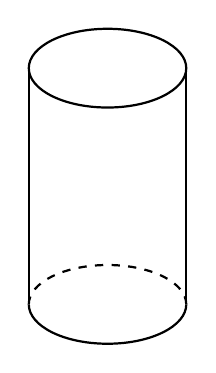
\begin{tikzpicture}[scale=0.5]
    \draw[thick] (0,0) ellipse (2cm and 1cm);
    \draw[thick] (-2,0) to (-2,-6);
    \draw[thick] (2,0) to (2,-6);
    \begin{scope}[shift={(0,-6)}]
      \draw[thick,dashed] (0:2cm and 1cm) arc (0:180:2cm and 1cm);
      \draw[thick] (180:2cm and 1cm) arc (180:360:2cm and 1cm);
    \end{scope}
  \end{tikzpicture}
$$
(that's supposed to look like a pipe!) and
$$
  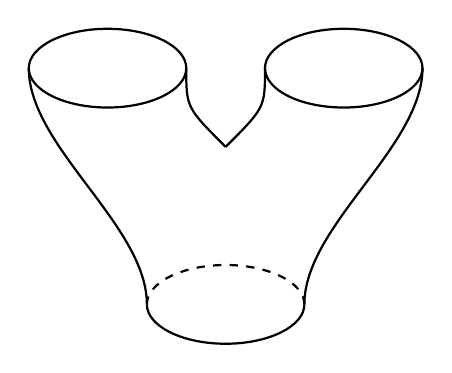
\begin{tikzpicture}[scale=0.5]
    \draw[thick] (-3,0) ellipse (2cm and 1cm);
    \draw[thick] (3,0) ellipse (2cm and 1cm);
    \draw[thick] (-5,0) .. controls (-5,-2) and (-2,-4) .. (-2,-6);
    \draw[thick] (5,0) .. controls (5,-2) and (2,-4) .. (2,-6);
    \draw[thick] (-1,0) .. controls (-1,-1) .. (0,-2);
    \draw[thick] (1,0) .. controls (1,-1) .. (0,-2);
    \begin{scope}[shift={(0,-6)}]
      \draw[thick,dashed] (0:2cm and 1cm) arc (0:180:2cm and 1cm);
      \draw[thick] (180:2cm and 1cm) arc (180:360:2cm and 1cm);
    \end{scope}
  \end{tikzpicture}
$$
--- that is, a cylinder and a "trinion" (or upside-down pair of pants)
--- we can combine them either "horizontally" like this:
$$
  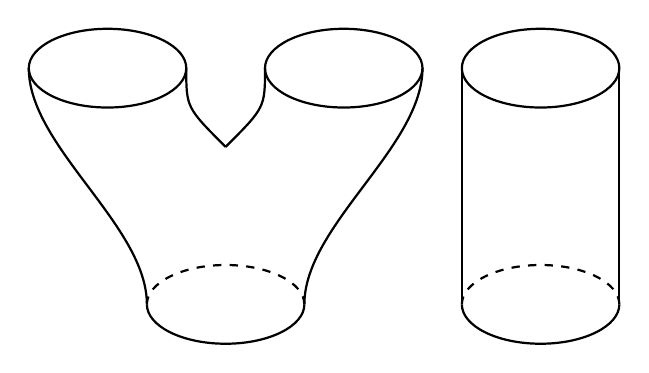
\begin{tikzpicture}[scale=0.5]
    \begin{scope}[shift={(8,0)}]
      \draw[thick] (0,0) ellipse (2cm and 1cm);
      \draw[thick] (-2,0) to (-2,-6);
      \draw[thick] (2,0) to (2,-6);
      \begin{scope}[shift={(0,-6)}]
        \draw[thick,dashed] (0:2cm and 1cm) arc (0:180:2cm and 1cm);
        \draw[thick] (180:2cm and 1cm) arc (180:360:2cm and 1cm);
      \end{scope}
    \end{scope}
    \draw[thick] (-3,0) ellipse (2cm and 1cm);
    \draw[thick] (3,0) ellipse (2cm and 1cm);
    \draw[thick] (-5,0) .. controls (-5,-2) and (-2,-4) .. (-2,-6);
    \draw[thick] (5,0) .. controls (5,-2) and (2,-4) .. (2,-6);
    \draw[thick] (-1,0) .. controls (-1,-1) .. (0,-2);
    \draw[thick] (1,0) .. controls (1,-1) .. (0,-2);
    \begin{scope}[shift={(0,-6)}]
      \draw[thick,dashed] (0:2cm and 1cm) arc (0:180:2cm and 1cm);
      \draw[thick] (180:2cm and 1cm) arc (180:360:2cm and 1cm);
    \end{scope}
  \end{tikzpicture}
$$
or "vertically" like this:
$$
  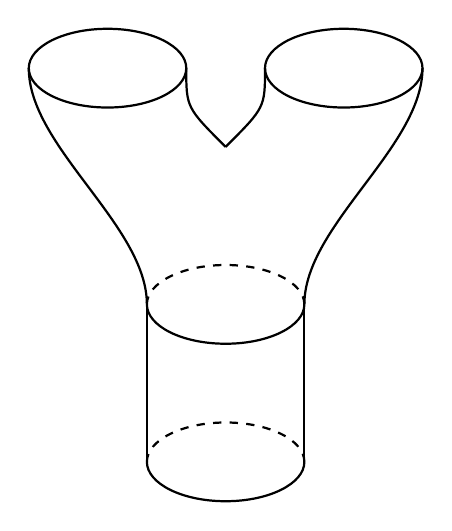
\begin{tikzpicture}[scale=0.5]
    \draw[thick] (-3,0) ellipse (2cm and 1cm);
    \draw[thick] (3,0) ellipse (2cm and 1cm);
    \draw[thick] (-5,0) .. controls (-5,-2) and (-2,-4) .. (-2,-6);
    \draw[thick] (5,0) .. controls (5,-2) and (2,-4) .. (2,-6);
    \draw[thick] (-1,0) .. controls (-1,-1) .. (0,-2);
    \draw[thick] (1,0) .. controls (1,-1) .. (0,-2);
    \begin{scope}[shift={(0,-6)}]
      \draw[thick,dashed] (0:2cm and 1cm) arc (0:180:2cm and 1cm);
      \draw[thick] (180:2cm and 1cm) arc (180:360:2cm and 1cm);
    \end{scope}
    \draw[thick] (-2,-6) to (-2,-10);
    \draw[thick] (2,-6) to (2,-10);
    \begin{scope}[shift={(0,-10)}]
      \draw[thick,dashed] (0:2cm and 1cm) arc (0:180:2cm and 1cm);
      \draw[thick] (180:2cm and 1cm) arc (180:360:2cm and 1cm);
    \end{scope}
  \end{tikzpicture}
$$

Corresponding to each spacetime we have a ``time evolution operator''
--- a linear operator that describes how states going in one end pop out
the other, ``evolved in time''. And corresponding to horizontal and
vertical composition of spacetimes we have two ways to compose
operators: horizontal composition usually being called ``tensor
product'', and vertical composition being called simply ``composition''.
These two ways satisfy some compatibility conditions, as well.

Now if one has read a bit about \(n\)-categories and/or ``extended''
topological quantum field theories, one already knows that this is just
the tip of the iceberg. If we allow ourselves to cut spacetimes into
smaller bits --- e.g., pieces with ``corners'', such as tetrahedra or
their higher-dimensional kin --- one gets more possible ways of
composing operators, and more compatibility conditions. These become
algebraically rather sophisticated, but luckily, there is a huge amount
of evidence that existing TQFTs extend to more sophisticated structures
of this sort, through a miraculous harmony between algebra and topology.

This leads to some interesting new concepts when it comes to the
physical interpretation of extended TQFTs. As Crane described in his
talk (see also his papers listed in \protect\hyperlink{week2}{``Week
2''}, \protect\hyperlink{week23}{Week 23} and
\protect\hyperlink{week56}{Week 56}), in a 4-dimensional extended TQFT
one expects the following sort of thing. If we think of an ``observer''
as a 3-manifold with boundary --- imagine a person being the 3-manifold
and his skin being the boundary, if one likes --- the extended TQFT
should assign to his boundary a ``Hilbert category'' or ``2-Hilbert
space''. This is the categorical analog of a Hilbert space. In other
words, just as a Hilbert space is a \emph{set} in which you can
\emph{sum} things and \emph{multiply} them by \emph{complex numbers},
and get \emph{complex numbers} by taking \emph{inner products} of
things, a 2-Hilbert space is an analogous structure in which every term
surrounded by asterisks is replaced by its analog one step up the
categorical ladder. This means: \[
  \begin{aligned}
    \text{set} &\to \text{category}
  \\\text{sum} &\to \text{direct sum}
  \\\text{multiply} &\to \text{tensor}
  \\\text{complex numbers} &\to \text{vector spaces}
  \\\text{inner products} &\to \text{homs}
  \end{aligned}
\]

There's a good chance that you know the analogy between numbers and
vector spaces: just as you can add numbers and multiply them, you can
take direct sums and tensor products of vector spaces, and many of the
same rules still apply (in a somewhat more sophisticated form, because
laws that were equations are now isomorphisms). A little less familiar
is the analogy between inner products and ``homs''. Given two vectors
\(v\) and \(w\) in a Hilbert space you can take the inner product
\(\langle v,w\rangle\) and get a number; similarly, given two
(finite-dimensional) Hilbert spaces \(V\) and \(W\) you can form
\(\mathrm{hom}(V,W)\) --- that is, the set of all linear maps from \(V\)
to \(W\) --- and get a Hilbert space. The same thing works in any
``2-Hilbert space''.

The most basic example of a 2-Hilbert space would be Hilb, the category
of finite-dimensional Hilbert spaces, but also \(\mathsf{Reps}(G)\), the
category of finite-dimensional unitary representations of a finite
group. (Similar remarks hold for quantum groups at root of unity.) Just
as the inner product is linear in one argument and conjugate-linear in
the other, ``\(\mathrm{hom}\)'' behaves nicely under direct sums in each
argument, but each argument behaves a bit differently under tensor
product, so one can say it's ``linear'' in one and ``conjugate-linear''
in the other.

So anyway, just as in a 4d TQFT a 3-manifold \(M\) determines a Hilbert
space \(Z(M)\), and a 4-manifold \(N\) with boundary equal to \(M\)
determines a vector \(Z(N)\) in \(Z(M)\), something similar happens in
an extended TQFT. (For experts, here I'm really talking about
``unitary'' TQFTs and extended TQFTs --- these are the physically
sensible ones.) Namely, a ``skin of observation'' or 2-manifold \(S\)
determines a 2-Hilbert space \(Z(S)\), and an ``observer'' or 3-manifold
\(M\) with boundary equal to \(S\) determines an object in \(Z(S)\).
Now, given two observers \(M\) and \(M'\) with the same ``skin'' --- for
example, the observer ``you'' and the observer ``everything in the world
except you'' --- one gets two objects \(Z(M)\) and \(Z(M')\) in
\(Z(S)\), so one can form the ``inner product''
\(\mathrm{hom}(Z(M),Z(M'))\), which is a Hilbert space. This is
\emph{your} Hilbert space for describing states of \emph{everything in
the world except you}. Note that we are using the term ``observer'' here
in a somewhat whimsical sense; in particular, every region of space
counts as an observer in this game, so we can flip things around and
form the inner product \(\mathrm{hom}(Z(M'),Z(M))\), which is the
Hilbert space that \emph{everything in the world except you} can use to
describe states of \emph{you}. These two Hilbert spaces, with roles
reversed, are conjugate to each other (using an obvious but perhaps
slightly unfamiliar definition of ``conjugate'' Hilbert space), so
they're pretty much the same.

Now this may at first seem weird, but if you think about it, it becomes
a bit less so. Of course, all of this stuff simply follows from the
notion of a unitary extended TQFT, and whether the actual laws of
physics are given by such a structure is a separate issue. But there is
clearly a lot of relevance to the ``holographic hypothesis'' and Lee
Smolin's more mathematical version of that hypothesis, as sketched in
\protect\hyperlink{week57}{``Week 57''}. The basic idea, there as here,
is that we are concentrating our attention on the things about a system
that can be measured at its boundary, and what we measure there can be
either thought of describing the state of the ``inside'' or dually the
``outside''.

I think if I go out on a limb here, and rhapsodize a bit, the point
might be clearer: but don't take this too seriously. Namely: all of the
stuff you see, hear, and otherwise observe about the world --- which
seems to be ``information about the outside'' --- is also stuff going on
in your brain, hence ``information about the inside''. What this stuff
really is, of course, is \emph{correlations} between the inside and the
outside. This is the reason for the duality between observer and
observed mentioned above. Note: we need not worry here whether or not
there's ``really'' a lot more going on outside than what you observe.
The point is simply that everything \emph{you} observe about what's
going on in the world outside is correlated to stuff that the world
could observe about what is going on in you. (Maybe.)

I should perhaps also add that the mathematicians are getting a bit
behind on the job of developing the ``higher linear algebra'' needed to
support this sort of physics. So it's a bit hard to point to a good
reference for all this 2-Hilbert space stuff. I'm slowly writing a paper
on it, but for now the best sources seem to be Kapranov and Voevodsky's
work on 2-vector spaces:

\begin{enumerate}
\def\labelenumi{\arabic{enumi})}
\setcounter{enumi}{1}
\tightlist
\item
  M. Kapranov and V. Voevodsky, ``2-Categories and Zamolodchikov
  tetrahedra equations'', in \emph{Proc. Symp. Pure Math.} \textbf{56},
  Part 2 (1994), AMS, Providence, pp.~177--260.
\end{enumerate}

(see also \protect\hyperlink{week4}{``Week 4''}) Dan Freed's work on
higher algebraic structures in gauge theory
(\protect\hyperlink{week12}{``Week 12''},
\protect\hyperlink{week48}{``Week 48''}), and David Yetter's new paper:

\begin{enumerate}
\def\labelenumi{\arabic{enumi})}
\setcounter{enumi}{2}
\tightlist
\item
  David Yetter, ``Categorical linear algebra: a setting for questions
  from physics and low-dimensional topology'', Kansas U. preprint,
  available as \texttt{http://math.ucr.edu/home/baez/yetter.pdf} and
  \texttt{http://math.ucr.edu/home/baez/yetter.ps}
\end{enumerate}

This treats 2-vector spaces in a very beautiful way, but not 2-Hilbert
spaces. Definitely worth reading for anyone interested in this sort of
thing!

While visiting Porto, I managed somehow to miss talking to Eugenia Cesar
de Sa, which was really a pity because she was the one who developed the
way of describing 4-manifolds that Broda (see
\protect\hyperlink{week9}{``Week 9''}, \protect\hyperlink{week10}{``Week
10''}) used to construct a 4-dimensional TQFT. This TQFT was later shown
by Roberts (see \protect\hyperlink{week14}{``Week 14''}) to be
isomorphic to that described by Crane and Yetter using a state sum model
--- i.e., by a discrete analog of a path integral in which one chops
spacetime up into 4-dimensional ``hypertetrahedra'' (better known as
4-simplices!), labels their 2d and 3d faces by spins, and sums over
labellings. Her work is cited in the Broda reference in
\protect\hyperlink{week17}{``Week 17''}, but I managed luckily to get a
copy of her thesis:

\begin{enumerate}
\def\labelenumi{\arabic{enumi})}
\setcounter{enumi}{3}
\tightlist
\item
  Eugenia Cesar de Sa, \emph{Automorphisms of 3-manifolds and
  representations of 4-manifolds}, Ph.D.~thesis, University of Warwick,
  1977.
\end{enumerate}

This should let me learn more about 4-dimensional topology, a
fascinating subject on which I'm woefully ignorant.

One reason why Broda's work, and thus de Sa's, is interesting to me, is
that people have suspected for a while that the Crane-Yetter-Broda
theory, which is constructed purely combinatorially, is isomorphic to BF
theory with cosmological term. BF theory (see
\protect\hyperlink{week36}{``Week 36''}) is a 4-dimensional field theory
that can be described starting from a Lagrangian in the traditional
manner of physics. The theory ``with cosmological term'' can be regarded
as a baby version of quantum gravity with nonzero cosmological constant,
a baby version having only one state, the ``Chern-Simons state''. As I
discussed in \protect\hyperlink{week56}{``Week 56''}, it's this
Chern-Simons state that plays a key role in Smolin's attempt to
``exactly solve'' quantum gravity. Thus I suspect that BF theory is a
good thing to understand really well. Recently I showed in

\begin{enumerate}
\def\labelenumi{\arabic{enumi})}
\setcounter{enumi}{4}
\tightlist
\item
  John Baez, ``4-dimensional BF theory with cosmological term as a
  topological quantum field theory'', available as
  \href{http://xxx.lanl.gov/abs/q-alg/9507006}{\texttt{q-alg/9507006}}.
\end{enumerate}

that the Crane-Yetter-Broda theory is indeed isomorphic as a TQFT to a
certain BF theory. With a bit more work, this should give us a state sum
model for the BF theory that's a baby version of quantum gravity in 4
dimensions. This should come in handy for studying Smolin's hypothesis
and its ramifications.

\begin{enumerate}
\def\labelenumi{\arabic{enumi})}
\setcounter{enumi}{5}
\tightlist
\item
  Timothy Porter, ``TQFTs from homotopy \(n\)-types'', University of
  Wales, Bangor preprint, available at
  \texttt{http://www.bangor.ac.uk/\textasciitilde{}mas013/preprint.html}
\end{enumerate}

The Dijkgraaf-Witten model is an n-dimensional TQFT one gets from a
finite group \(G\). It's given by a really simple state sum model. Chop
your manifold into simplices; then the allowed ``states'' are just
labellings of the edges with elements of \(G\) subject to the constraint
that the product around any triangle is \(1\). You can think of a
labelling as a kind of ``connection'' that tells you how to parallel
transport along the edges, and the constraint says the connection is
flat. Expectation values of physical observables are then computed as
sums over these states. In fact, this TQFT is a baby version of BF
theory \emph{without} cosmological constant. A toy model of a toy model
of quantum gravity, in other words: the classical solutions of BF theory
without cosmological constant are just flat connections on some G-bundle
where G is a Lie group, while the Dijkgraaf-Witten model does something
similar for a finite group.

In a previous paper (see \protect\hyperlink{week54}{``Week 54''}) Porter
studied the Dijkgraaf-Witten model and a generalization of it due to
Yetter that allows one to label faces with things too\ldots{} one can
think of this generalization as allowing ``curvature'', because the
product of elements of G around a triangle need no longer be \(1\);
instead, it's something determined by the labelling of the face.

\begin{enumerate}
\def\labelenumi{\arabic{enumi})}
\setcounter{enumi}{6}
\tightlist
\item
  David Yetter, ``TQFTs from homotopy 2-types'', \emph{Journal of Knot
  Theory and its Ramifications} \textbf{2} (1993), 113--123.
\end{enumerate}

In his new paper Porter takes this idea to its logical conclusion and
constructs analogous theories that allow labellings of simplices in any
dimension. Technically, the input data is no longer just a finite group,
but a finite simplicial group \(G\).

What's a simplicial group? It's a wonderful thing; using the
``internalization'' trick I've referred to in some previous Finds, all I
need to say is that it's a simplicial object in the category of groups.
A simplicial set is a bunch of sets, one for each natural number,
together with a bunch of ``face'' and ``degeneracy'' maps satisfying the
same laws that the face and degeneracy maps do for a simplex. (Students
of singular or simplicial homology will know what I'm talking about.)
Similarly, a simplicial group is a bunch of \emph{groups}, together with
a bunch of of ``face'' and ``degeneracy'' \emph{homomorphisms}
satisfying the same laws.

A triangulated manifold gives a simplicial set in an obvious way, and
from any simplicial set one can obtain a simplicial groupoid (like a
simplicial group, but with groupoids instead!) called its ``loop
groupoid''. The sort of labellings Porter considers are homomorphisms
from this simplicial groupoid to the given simplicial group G.

I will refrain from trying to say what all this has to do with homotopy
\(n\)-types. Nonetheless, from a pure mathematics point of view, that's
the most exciting aspect of the whole business! Part of the puzzle about
TQFTs is their relation to traditional algebraic topology (and
not-so-traditional algebraic topology like nonabelian cohomology,
\(n\)-stacks, etc.), and this work serves as a big clue about that
relationship.

\begin{center}\rule{0.5\linewidth}{0.5pt}\end{center}
\hypertarget{week59}{%
\section{August 3, 1995}\label{week59}}

\begin{quote}
\emph{As you crack your eyes one morning your reason is assaulted by a}
\emph{strange sight. Over your head, humming quietly, there floats a}
\emph{monitor, an ethereal otherworldly screen on which is written a
curious} \emph{message. "I am the Screen of ultimate Truth. I am bulging
with} \emph{information and ask nothing better than to be allowed to
impart it."}
\end{quote}

It would be nice if more math books started with something
attention-grabbing like this. In fact, it appears near the beginning of

\begin{enumerate}
\def\labelenumi{\arabic{enumi})}
\tightlist
\item
  Geoffrey M. Dixon, \emph{Division Algebras: Octonions, Quaternions,
  Complex Numbers and the Algebraic Design of Physics}, Springer Verlag,
  1994.
\end{enumerate}

Dixon is convinced that the details of the Standard Model of particle
interactions can be understood better by taking certain mathematical
structures very seriously. There are very few algebras over the reals
where we can divide by nonzero elements: if we demand associativity and
commutativity, just the reals themselves and the complex numbers. If we
drop the demand for commutativity, we also get a 4-dimensional algebra
called the quaternions, invented by Hamilton. If in addition we drop the
demand for associativity, and ask only that our algebra be
``alternative'', we also get an 8-dimensional algebra called the
octonions, or Cayley numbers. (I'll say what ``alternative'' means in
\protect\hyperlink{week61}{``Week 61''}) Clearly these are very special
structures, and also clearly they play an important role in
physics\ldots{} or do they?

Well, few people doubt that the real numbers are fundamental to physics
(though some advocates of the discrete might prefer the integers), and
with emergence of quantum theory, if not sooner, the basic role of the
complex numbers also became clear. Hamilton discovered the quaternions
in the 1800s, and used them to formulate a beautiful theory of rotations
in 3-dimensional space. They fell out of favor somewhat when the vectors
of Gibbs proved simpler for many purposes, but their deeper importance
became clear when people started studying spin: indeed, the Pauli
matrices so important in physics are closely related to the quaternions,
and it is the group of unit quaternions, \(SU(2)\), rather than the
group of rotations in 3d space, \(SO(3)\), which turns out to be the
symmetry group whose different representations correspond to particles
of different spin. But what about the octonions?

Well, there are not too many places in physics yet where the octonions
reach out and grab one with the force the reals, complexes, and
quaternions do. But they are certainly out there, they have a certain
beauty to them, and they are the natural stopping-point of a certain
finite sequence of structures, so it is natural for people of a certain
temperament to believe that they are there for a reason. Dixon makes a
passionate case for this in the beginning of his book.

Suppose you were confronted with the Screen of Truth. What would you ask
it? Dixon, being a physicist, naturally fantasizes asking it why the
universe is the way it is! What kind of answer could this possibly have?
Perhaps there is only one consistent way for things to be, and
mathematics, with its unique and beautiful structures that are pure
expressions of logical necessity, is trying to tell us something about
this?

On the one hand this seems outrageous\ldots{} especially to the
hard-nosed pragmatist or empiricist in us. It seems old-fashioned,
naive, and too good to be true. On the other hand, the universe
\emph{is} outrageous! It's outrageous that it exists in the first place,
and doubly outrageous that it has the particular physical laws it does
and no others. It has only been through the old-fashioned, naive belief
that we can understand it using mathematics that we discovered what we
have of its physical laws. So maybe eventually we \emph{will} see that
the basic structures of mathematics determine, in some mysterious sense,
all the basic laws of physics. Or maybe we won't. In either case, there
is a long way yet to go. As Dixon's Screen of Truth comments, before it
departs:

\begin{quote}
``Do you believe that were I to explain as much of what I know as you''
``could comprehend that you would recognize it, that you would say, oh''
``yes, this is but an extension of what we have already done, and
though'' ``the mathematics is broader, the principles deeper, I am not
surprised?'' ``Do you think you have asked even a fraction of the
questions you need'' ``to ask?''
\end{quote}

Anyway, it is at least worth considering all the beautiful mathematical
structures one runs into for their potential importance. For example,
the octonions.

In order to write this week's Finds, I needed to learn a little about
the octonions. I wanted some good descriptions of the octonions, that
hopefully would ``explain'' them or at least make them easy to remember.
So I asked for help on sci.physics.research, and I got some help from
Greg Kuperberg, Ezra Getzler, Matthew Wiener, and Alexander Vlasov.
After a while Geoffrey Dixon got wind of this and referred me to his
work! I'll probably talk to him later this summer when I go back to
Cambridge Massachusetts, and hopefully I'll learn more about octonions
and the like.

But for now let me just give a quick beginner's introduction to the
octonions. A lot of this appears in

\begin{enumerate}
\def\labelenumi{\arabic{enumi})}
\setcounter{enumi}{1}
\tightlist
\item
  William Fulton and Joe Harris, \emph{Representation Theory --- a First
  Course}, Springer Verlag, Berlin, 1991.
\end{enumerate}

I should add that this book is a very good place to learn about Lie
groups, Lie algebras, and their representations\ldots{} I wish I had
taken a course based on this book when I was in grad school!

Let's start with the real numbers. Then the complex number \[a+bi\] can
be thought of as a pair \[(a,b)\] of real numbers. Addition is done
component-wise, and multiplication goes like this:
\[(a,b)(c,d) = (ac - db,da + bc)\] We can also define the conjugate of a
complex number by \[(a,b)^* = (a,-b).\] Now that we have the complex
numbers, we can define the quaternions in a similar way. A quaternion
can be thought of as a pair \[(a,b)\] of complex numbers. Addition is
component-wise and multiplication goes like this
\[(a,b)(c,d) = (ac - d^*b, da + bc^*)\] This is just like how we defined
multiplication of complex numbers, but with a couple of conjugates
(\({}^*\)'s) thrown in. To emphasize how similar the two multiplications
are, we could have included the conjugates in the first formula, since
the conjugate of a real number is just itself.

We can also define the conjugate of a quaternion by
\[(a,b)^* = (a^*,-b).\] The game continues! Now we can define an
octonion to be a pair of quaternions; as before, we add these
component-wise and multiply them as follows:
\[(a,b)(c,d) = (ac - d^*b, da + bc^*).\] One can also define the
conjugate of an octonion by \[(a,b)^* = (a^*,-b).\] Why do the real
numbers, complex numbers, quaternions and octonions have multiplicative
inverses? I take it as obvious for the real numbers. For the complex
numbers, you can check that \[(a,b)^* (a,b) = (a,b) (a,b)^* = K (1,0)\]
where \(K\) is a real number called the ``norm squared'' of \((a,b)\).
The multiplicative identity for the complex numbers is \((1,0)\). This
means that the multiplicative inverse of \((a,b)\) is \((a,b)^*/K\). You
can check that the same holds for the quaternions and octonions!

This game of getting new algebras from old is called the
``Cayley-Dickson'' construction. Of course, the fun we've had so far
should make you want to keep playing this game and develop a
16-dimensional algebra, the ``hexadecanions,'' consisting of pairs of
octonions equipped with the same sort of multiplication law. What do you
get? Why aren't there multiplicative inverses anymore? I haven't
checked, because this is my summer vacation! I am learning about
octonions just for fun, since I just finished writing some rather
technical papers, and my idea of fun does not presently include
multiplying two hexadecanions together to see why the norm-squared law
\((a,b) (a,b)^* = (a,b)^* (a,b) = K (1,0)\) breaks down. But I'm sure
someone out there will enjoy doing this\ldots{} and I'm sure someone
else out there has already done it! So they should let me know what
happens. There is something out there called ``Pfister forms'', which I
think might be related.

{[}Toby Bartels did some nice work on hexadecanions in response to the
above challenge, which appears at the end of this article.{]}

Now if we unravel the above definition of quaternions, by writing the
quaternion \((a+bi,c+di)\) as \(a+bi+cj+dk\), we see that the
multiplication law is \[i^2 = j^2 = k^2 = -1,\] and
\[ij = -ji = k, \quad jk = -kj = i, \quad ki = -ik = j.\]

For more about the inner meaning of these rules, see
\protect\hyperlink{week5}{``Week 5''}. Similarly, we can unravel the
above definition of octonions by writing the octonion
\((a+bi+cj+dk,e+fi+gj+hk)\) as
\[a + b e_1 + c e_2 + d e_3 + e e_4 + f e_5 + g e_6 + h e_7.\] Note:
since mathematicians are very impersonal, they usually call these seven
dwarves \(e_1,\ldots,e_7\) instead of Sleepy, Grumpy, etc. as in the
Disney movie. Any one of these 7 guys times himself is \(-1\). Also, any
two distinct ones anticommute; for example, \(e_3 e_7 = -e_7 e_3\).
There is a nice way to remember how to multiply them using the ``Fano
plane''. This is a projective plane with 7 points, where by a
``projective plane'' I mean that any two points determine an abstract
sort of ``line'', which in this case consists of just 3 points, and any
two lines intersect in a point. It looks like this:
$$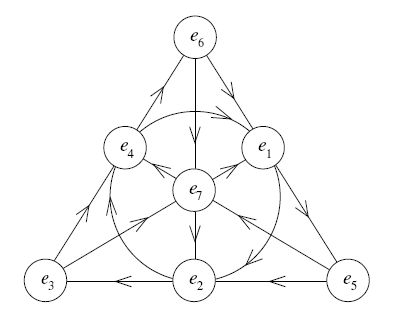
\includegraphics{../images/fano.jpg}$$

The ``lines'' are the 3 edges of the big triangle, the 3 lines going
through a vertex, the center and the midpoint of the opposite edge, and
the circle including \(e_1\), \(e_2\), and \(e_3\). All the ``lines''
are cyclically ordered, and that tells you how to multiply the seven
dwarves. For example, the line that's actually a circle goes clockwise,
so \(e_1 e_2 = e_4\), \(e_2 e_4 = e_1\), and \(e_4 e_1 = e_2\). The
lines that are edges of the big triangle also point clockwise, so for
example \(e_5 e_2 = e_3\), and cyclic permutations thereof, and
\(e_6 e_3 = e_4\). The lines that go through the center point from the
vertex to the midpoint of the opposite edge, so for example
\(e_3 e_7 = e_1\). I hope that made sense; you can work it out yourself,
of course.

My convention for numbering the seven dwarves in the picture above is
\emph{completely arbitrary}, so don't bother remembering it --- make up
your own if you prefer! The convention I chose looks sort of weird at
first, but it has a couple of endearing features:

\begin{itemize}
\tightlist
\item
  Index cycling: if \(e_i e_j = e_k\), then
  \(e_{i+1} e_{j+1} = e_{k+1}\).
\item
  Index doubling: if \(e_i e_j = e_k\), then \(e_{2i} e_{2j} = e_{2k}\).
\end{itemize}

Here we add and multiply \(\mod 7\). Index doubling corresponds to
rotating the Fano plane.

So those are the octonions in a nutshell. I should say a bit about how
they relate to triality for \(SO(8)\), the exceptional Lie group
\(G_2\), the group \(SU(3)\) which is so important in the study of the
strong force, and to lattices like \(E_8\), \(\Lambda 16\) and the Leech
lattice. But I will postpone that; for now you can consult Fulton and
Harris, and also various papers by Dixon:

\begin{enumerate}
\def\labelenumi{\arabic{enumi})}
\setcounter{enumi}{2}
\item
  Geoffrey Dixon, ``Octonion X-product orbits'', preprint available as
  \href{http://xxx.lanl.gov/abs/hep-th/9410202}{\texttt{hep-th/9410202}}.

  ``Octonion X-product and E\_8 lattices'', preprint available as
  \href{http://xxx.lanl.gov/abs/hep-th/9411063}{\texttt{hep-th/9411063}}.

  ``Octonions: \(E_8\) lattice to \(\Lambda 16\)'', preprint available
  as
  \href{http://xxx.lanl.gov/abs/hep-th/9501007}{\texttt{hep-th/9501007}}.

  ``Octonions: invariant representation of the Leech lattice'', preprint
  available as
  \href{http://xxx.lanl.gov/abs/hep-th/9504040}{\texttt{hep-th/9504040}}.

  ``Octonions: invariant Leech lattice exposed'', preprint available as
  \href{http://xxx.lanl.gov/abs/hep-th/9506080}{\texttt{hep-th/9506080}}.
\end{enumerate}

I am not presently in a position to assess these papers or Dixon's work
relating division algebras and the Standard Model, but hopefully
sometime I will be able to say a bit more.

Let me wrap up by saying a bit about the Leech lattice. As described in
my review of Conway and Sloane's book (\protect\hyperlink{week20}{``Week
20''}, there is a wonderful branch of mathematics that studies the
densest ways of packing spheres in n dimensions. Most of the results so
far concern lattice packings, packings in which the centers of the
spheres form a subset of \(\mathbb{R}^n\) closed under addition and
scalar multiplication by integers. When \(n = 8\), the densest known
packing is given by the so-called \(E_8\) lattice. In
\protect\hyperlink{week20}{``Week 20''} I described how to get this
lattice using the quaternions and the icosahedron. Briefly, it goes as
follows. The group of rotational symmetries of the icosahedron (not
counting reflections) is a subgroup of the rotation group \(SO(3)\)
containing 60 elements. As mentioned above, \(SO(3)\) has as a double
cover the group \(SU(2)\) of unit quaternions. So there is a 120-element
subgroup of \(SU(2)\) consisting of elements that map to elements of
\(SO(3)\) that are symmetries of the icosahedron. Now form all integer
linear combinations of these 120 special elements of \(SU(2)\). We get a
subring of the quaternions known as the "icosians'\,'.

We can think of icosians as special quaternions, but we can also think
of them as special vectors in \(\mathbb{R}^8\), as follows. Every
icosian is of the form
\[(a + \sqrt{5} b) + (c + \sqrt{5} d)i + (e + \sqrt{5} f)j + (g + \sqrt{5} h)k\]
with \(a,b,c,d,e,f,g,h\) rational --- but not all rational values of
\(a,\ldots,h\) give icosians. The set of all vectors
\(x = (a,b,c,d,e,f,g,h)\) in \(\mathbb{R}^8\) that correspond to
icosians in this way is the \(E_8\) lattice!

The Leech lattice is the densest known packing in 24 dimensions. It has
all sorts of remarkable properties. Here is an easy way to get ones
hands on it. First consider triples of icosians \((x,y,z)\). Let \(L\)
be the set of such triples with \[x = y = z \mod h\] and
\[x + y + z = 0 \mod h^*\] where \(h\) is the quaternion
\((-\sqrt{5} + i + j + k)/2\). Since we can think of an icosian as a
vector in \(\mathbb{R}^8\), we can think of \(L\) as a subset of
\(\mathbb{R}^{24}\). It is a lattice, and in fact, it's the Leech
lattice! I have a bit more to say about the Leech lattice in
\protect\hyperlink{week20}{``Week 20''}, but the real place to go for
information on this beast is Conway and Sloane's book. It turns out to
be related to all sorts of other "exceptional'\,' algebraic structures.
People have found uses for many of these in string theory, so if string
theory is right, maybe they are important in physics. Personally, I want
to understand them more deeply as pure mathematics before worrying too
much about their applications to physics.

\begin{center}\rule{0.5\linewidth}{0.5pt}\end{center}

Here is what Toby Bartels wrote:

\begin{quote}
From: Toby Bartels Subject: Re: why hexadecanions have no inverses To:
John Baez Date: Sun, 20 Aug 1995
\end{quote}

\begin{quote}
I spent a couple days thinking about why hexadecanions have no inverses,
and the first thing I want to say about it is that they do. However,
these inverses are of limited applicability, because the hexadecanions
are not a division algebra. A division algebra allows you to conclude,
given \(x y = 0\), that \(x\) or \(y\) is \(0\). If your algebra has
inverses, you might try to multiply this equation by the inverse of
\(x\) or \(y\) (whichever one isn't \(0\)) to prove the other is \(0\),
but this only works if the algebra is associative. Since the octonions
and hexadecanions aren't associative, there's no reason (yet) to think
either of these is a division algebra. It turns out that the octonions
are a division algebra, despite not being associative, but the
hexadecanions aren't.

Why aren't the hexadecanions a division algebra? Because the real
numbers aren't of characteristic 2. Allow me to explain.

I will prove below that the \(2^n\) onions are a division algebra only
if the \(2^{n-1}\) onions are associative. So, the question becomes: why
aren't the octonions associative? Well, I've found a proof that \(2^n\)
onions are associative only if \(2^{n-1}\) onions are commutative. So,
why aren't the quaternions commutative? Again, I have a proof that
\(2^n\) onions are commutative only if \(2^{n-1}\) onions equal their
own conjugates. So, why don't the complex numbers equal their own
conjugates? I have a proof that \(2^n\) onions do equal their own
conjugates, but it works only if the \(2^{n-1}\) onions are of
characteristic 2. The real numbers are not of characteristic 2, so the
complex numbers don't equal their own conjugates, so the quaternions
aren't commutative, so the octonions aren't associative, so the
hexadecanions aren't a division algebra.

I require a few identities about conjugates that hold for all \(2^n\)
onions: \((x^*)^* = x\), \((x + y)^* = x^* + y^*\), and
\((x y)^* = y^* x^*\). (If these identities are reminiscent of
identities for transposes of matrices, it is no coincidence.) I will
prove these by induction. That is, if an identity holds for \(2^{n-1}\)
onions, I show it holds for \(2^n\) onions. Since they hold trivially
for the reals (\(n = 0\)), they hold for all.

\[((a, b)^*)^* = (a^*, -b)^* = ((a^*)^*, -(-b)).\] By the induction
hypothesis and the nature of addition (an Abelian group),
\[((a^*)^*, -(-b)) = (a, b).\]
\[((a, b) + (c, d))^* = (a + c, b + d)^* = ((a + c)^*, -(b + d)).\] By
the induction hypothesis and addition again,
\[((a + c)^*, -(b + d)) = (a^* + c^*, -b + -d) = (a^*, -b) + (c^*, -d) = (a, b)^* + (c, d)^*.\]

The next proof needs the distribution of multiplication over addition.
\[(a, b) ((c, d) + (e, f)) = (a, b) (c + e, d + f) = (a (c + e) - (d + f)^* b, (d + f) a + b (c + e)^*).\]
By the induction hypothesis and the identity immediately above, \[
  \begin{gathered}
    (a (c + e) - (d + f)^* b, (d + f) a + b (c + e)^*)
  \\= (a c + a e - d^* b - f^* b, d a + f a + b c^* + b e^*)
  \\= (a c - d^* b, d a + b c^*) + (a e - f^* b, f a + b e^*)
  \\= (a, b) (c, d) + (a, b) (e, f).
  \end{gathered}
\] Also, \[
  \begin{gathered}
    ((a, b) + (c, d)) (e, f)
  \\= (a + c, b + d) (e, f)
  \\= ((a + c) e - f^* (b + d), f (a + c) + (b + d) e^*).
  \end{gathered}
\] By the induction hypothesis again, \[
  \begin{gathered}
    ((a + c) e - f^* (b + d), f (a + c) + (b + d) e^*)
  \\= (a e + c e - f^* b - f^* d, f a + f c + b e^* + d e^*)
  \\= (a e - f^* b, f a + b e^*) + (c e - f^* d, f c + d e^*)
  \\= (a, b) (e, f) + (c, d) (e, f).
  \end{gathered}
\]

\[((a, b) (c, d))^* = (a c - d^* b, d a + b c^*)^* = ((a c - d^* b)^*, -(d a + b c^*)).\]
Using the induction hypothesis and each of the above identities, \[
  \begin{gathered}
    ((a c - d^* b)^*, -(d a + b c^*))
  \\= (c^* a^* - (-b)^* (-d), -d a + (-b) c^*)
  \\= (c^*, -d) (a^*, -b)
  \\= (c, d)^* (a, b)^*.
  \end{gathered}
\]

In light of the above identities, if I ever come across, say,
\((x y^* + z)^*\), I'll simply write \(y x^* + z^*\) without a moment's
hesitation.

Since inductive proofs have been so useful, I'll use one to prove that
\(2^n\) onions always have inverses. First, I'll extend the method in
John's article, beginning with an inductive proof that \(x x^* = x^* x\)
is real. \[(a, b) (a, b)^* = (a, b) (a^*, -b) = (a a^* + b^* b, 0),\]
and \[(a, b)^* (a, b) = (a^*, -b) (a, b) = (a^* a + b^* b, 0).\] The
inductive hypothesis states that both \(a^* a = a a^*\) and \(b^* b\)
are real, so \((a, b) (a, b)^* = (a, b)^* (a, b)\) is real. Since the
sum of a positive real and a nonnegative real is positive, I can take
this as a proof by induction that \(x x^* = x^* x\) is not only real,
but is also positive unless \(x = 0\) (which will be important). All you
have to do now is check that these things are true of the \(2^0\)
onions, and they are, quite trivially (since the \(2^0\) onions are the
reals).

Since the \(2^n\) onions are always a vector space over the reals (as
mentioned in John's article),
\[x (x^* / (x x^*)) = (x x^*) / (x x^*) = 1.\] Since one can always
divide by the real \(x x^*\), the inverse of \(x\) is \(x^* / (x x^*)\)
in any \(2^n\) onion algebra.

To continue with the streak of inductive proofs, I will now try to prove
that the \(2^n\) onions are always a division algebra. (I will fail.)
Assume \[0 = (0, 0) = (a, b) (c, d) = (a c - d^* b, d a + b c^*).\] This
gives the system of equations \[a c - d^* b = 0 = d a + b c^*.\]
Multiplying,
\[(a c) c^* - (d^* b) c^* = 0 c^* = 0 = d^* 0 = d^* (d a) + d^* (b c^*).\]
If \(2^{n-1}\) onions are associative, I can add the equations to get
\[a (c c^*) + (d^* d) a = 0.\] Since \(c c^*\) and \(d^* d\) are real,
they commute with \(a\), and the division algebra nature of \(2^{n-1}\)
onions allows me to conclude that \(c c^* + d^* d = 0\) (which implies
\(c = d = 0\) in light of positive definiteness) or that \(a = 0\) (from
which the original equation gives \(b = 0\)). Thus, the octonions are a
division algebra (since the quaternions are associative), but the
hexadecanions aren't (since the octonions aren't associative).

(If you're reading carefully, you realize that I haven't really proved
that the hexadecanions aren't a division algebra. I've failed to prove
that they are, but that's not the same thing. When I first wrote this, I
wasn't reading carefully; I will return to plug this hole later.)

Thus, the \(2^n\) onions are a division algebra iff the \(2^{n-1}\)
onions are a division algebra and are associative. So, let's try to
prove associativity of \(2^n\) onions by induction. \[
  \begin{gathered}
    ((a, b) (c, d)) (e, f)
  \\= (a c - d^* b, d a + b c^*) (e, f)
  \\= ((a c - d^* b) e - f^* (d a + b c^*), f (a c - d^* b) + (d a + b c^*) e^*)
  \\=((ac)e - (d^* b)e - f^* (da) - f^* (b c^*), f(ac) - f(d^* b) + (da) e^* + (b c^*) e^*).
  \end{gathered}
\] On the other hand, \[
  \begin{gathered}
    (a, b) ((c, d) (e, f))
  \\= (a, b) (c e - f^* d, f c + d e^*)
  \\= (a (c e - f^* d) - (f c + d e^*)^* b, (f c + d e^*) a + b (c e - f^* d)^*)
  \\= (a(ce) - a(f^* d) - (c^* f^*)b - (e d^*)b, (fc)a + (d e^*)a + b(e^* c^*) - b(d^* f)).
  \end{gathered}
\] Assuming the induction hypothesis that \(2^{n-1}\) onions are
associative, these are equal in general iff \(2^{n-1}\) onions also are
commutative.

Thus, \(2^n\) onions are associative iff \(2^{n-1}\) onions are
associative and are commutative. So, let's try to prove commutativity of
\(2^n\) onions by induction.
\[(a, b) (c, d) = (a c - d^* b, d a + b c^*).\] On the other hand,
\[(c, d) (a, b) = (c a - b^* d, b c + d a^*).\] Assuming the induction
hypothesis that \(2^{n-1}\) onions are commutative, these are equal in
general iff \(2^{n-1}\) onions also equal their own conjugates.

Thus, \(2^n\) onions are commutative iff \(2^{n-1}\) onions are
commutative and equal their own conjugates. So, let's try to prove
conjugate equality of \(2^n\) onions by induction. \[(a, b) = (a, b).\]
On the other hand, \[(a, b)^* = (a^*, -b).\] Assuming the induction
hypothesis that \(2^{n-1}\) onions equal their own conjugates, these are
equal in general iff \(2^{n-1}\) onions also have characteristic 2.
(\(b = -b\) means \(0 = b + b = 1 b + 1 b = (1 + 1) b = 2 b\); this is
true in general iff \(0 = 2\), which is what characteristic 2 means.)

Thus, \(2^n\) onions equal their own conjugates iff \(2^{n-1}\) onions
equal their own conjugates and have characteristic 2. Since the reals
don't have characteristic 2, there's no point in trying to prove
anything about that by induction. However, it's a general result that
any algebra has characteristic 2 if it has a superalgebra of
characteristic 2. Since the \(2^n\) onions are all superalgebras of the
reals (which means the reals are always isomorphic to a subset of the
\(2^n\) onions), none of the \(2^n\) onions can have characteristic 2 if
the reals don't.

In summary, the definition of the reals as the complete ordered field,
along with an initial definition that \(x^* = x\) in the reals, allows
trivial proofs that: they form a division algebra, they are associative,
they are commutative, and they equal their own conjugates, but they
don't have characteristic 2. (All of these, in fact, are true of any
ordered field with this definition of conjugate, complete or not.) From
this and the above considerations, the complex numbers form a division
algebra, are associative, and are commutative, but they neither equal
their own conjugates nor have characteristic 2. From this, the
quaternions form a division algebra and are associative, but they
neither are commutative, equal their own conjugates, nor have
characteristic 2. From this, the octonions form a division algebra but
they neither associative, are commutative, equal their own conjugates,
nor have characteristic 2. Finally, the hexadecanions neither form a
division algebra, are associative, are commutative, equal their own
conjugates, nor have characteristic 2.

At this point, I must return to the logical hole I mentioned earlier.
But I want to work with a different algebraic concept than a division
algebra; instead I will use (inspired by Doug Merrit's post to
\texttt{sci.physics.research}) what I guess is called `alternativity',
which says \(x (x y) = (x x) y\). I don't like putting alternativity
into the pattern, since associativity implies alternativity. All the
other properties (commutativity, conjugate equality, characteristic) are
logically independent in general. I'd like to prove that every
associative \(2^n\) onion algebra is alternative, just as I proved every
commutative one was associative, without its having been obvious to
begin with. Well, I will be disappointed even more badly later on.

Taking the conjugate of \(x (x y) = (x x) y\),
\[(y^* x^*) x^* = y^* (x^* x^*),\] so left alternativity implies right
alternativity, for \(2^n\) onions.

I require an additional general identity of \(2^n\) onions. Earlier, I
proved by induction that \(x x^*\) was real, but now I need the reality
of \(x + x^*\). Like everything else, this is proved by induction.
\[(a, b) + (a, b)^* = (a, b) + (a^*, -b) = (a + a^*, 0).\] Thus, if
\(a + a^*\) is real, \((a, b) + (a, b)^*\) is real. Since \(x + x^*\) is
real when \(x\) is real, \(x + x^*\) is real when \(x\) is any \(2^n\)
onion.

Now suppose we're working in an alternative \(2^n\) onion algebra.
\[x (x y) + x^* (x y) = (x + x^*) (x y).\] Since \(x + x^*\) is real, it
associates, so
\[x (x y) + x^* (x y) = ((x + x^*) x) y = (x x) y + (x^* x) y.\] Since
\(x (x y) = (x x) y\), \[x^* (x y) = (x^* x) y,\] which will be needed.

Let's attempt to prove by induction that \(2^n\) onions are always
alternative. \[
  \begin{gathered}
    (a, b) ((a, b) (c, d))
  \\= (a, b) (a c - d^* b, d a + b c^*)
  \\= (a (a c - d^* b) - (d a + b c^*)^* b, (d a + b c^*) a + b (a c - d^* b)^*)
  \\= (a(ac) - a(d^* b) - (a^* d^*)b - (c b^*)b, (da)a + (b c^*)a + b(c^* a^*) - b(b^* d)).
  \end{gathered}
\] Meanwhile, \[
  \begin{gathered}
    ((a, b) (a, b)) (c, d)
  \\= (a a - b^* b, b a + b a^*) (c, d)
  \\= ((aa)c - (b^* b)c - d^* (ba) - d^* (b a^*),d(aa) - d(b^* b) + (ba) c^* + (b a^*) c^*).
  \end{gathered}
\] These are indeed equal in general iff \(2^{n-1}\) onions are
associative.

The last sentence may not be immediately obvious. The induction
hypothesis and its corollaries leave us with
\(x (y z) + (x^* y) z = y (z x) + y (z x^*)\) as a necessary and
sufficient condition. It may not be clear that associativity implies
this, much less vice versa. However, the reality of \(x + x^*\) once
more enters the picture.
\[y (z x) + y (z x^*) = y (z (x + x^*)) = (x + x^*) (y z) = x (y z) + x^* (y z).\]
Thus, the condition becomes
\[x (y z) + (x^* y) z = x (y z) + x^* (y z),\] which is equivalent, in
the general case, to associativity.

To sum up the findings so far: For any n, the \(2^n\) onions form a
vector space over the reals. \(x + x^*\) and \(x x^*\) are real if \(x\)
is any \(2^n\) onion; additionally, \(x x^* = x^* x.\) Every \(2^n\)
onion has an inverse, which is a real multiple of its conjugate.
Conjugation is analogous to matrix transposition in that
\[(x^*)^* = x, (x + y)^* = x^* + y^*, and (x y)^* = y^* x^*.\]
Multiplication distributes over addition every time. For no n do all
\(2^n\) onions equal their own negatives. \(2^{n+1}\) onions equal their
own conjugates iff \(2^n\) onions equal their own conjugates and their
own negatives. all \(2^{n+1}\) onions commute iff all \(2^n\) onions
commute and equal their own conjugates. \(2^{n+1}\) onions are
associative iff \(2^n\) onions are associative and commutative.
\(2^{n+1}\) onions are alternative iff \(2^n\) onions are alternative
and associative. The \(2^n\) onions form a division algebra if they are
alternative.

I will be satisfied if I can prove the converse of the last statement.
In light of the results about alternativity, my original attempt to
prove that division of \(2^n\) onions requires associativity of
\(2^{n-1}\) onions looks even more convincing, (since alternativity of
\(2^{n-1}\) onions can be included in the induction hypothesis), but
it's still not valid. I still haven't shown that, if \(2^{n-1}\) onions
aren't alternative, there must be non0 \(2^n\) onions \(x\) and \(y\)
such that \(x y = 0\). There doesn't seem to be any reason why there
shouldn't be, but there just might happen not to be any. So, despite the
inelegance of it all, in order to prove that the hexadecanions aren't a
division algebra, I'm forced to exhibit non-\(0\) \(x\) and \(y\) such
that \(x y = 0\).

Just playing around, I found \[
  \begin{gathered}
    (e_1, e_4) (-1, e_5)
  \\= (e_1 (-1) - (e_5)* e_4, e_5 e_1 + e_4 (-1)*)
  \\= (-e_1 + e_5 e_4, e_5 e_1 - e_4).
  \end{gathered}
\] Since \(e_5 e_4 = (0, i) (0, 1) = (i, 0) = e_1\) and
\(e_5 e_1 = (0, i) (i, 0) = (0, i* i) = (0, 1) = e_4\),
\[(e_1, e_4) (-1, e_5) = (0, 0) = 0.\]

The \(2^n\) onions can't be a division algebra if the \(2^{n-1}\) onions
aren't. If \(x y = 0\) in the \(2^{n-1}\) onions,
\((x, 0) (y, 0) = (x y, 0) = (0, 0) = 0\). Thus, the octonions and below
are the only \(2^n\) onions to be division algebras. Still, I wish I had
a proof of this that didn't require the ugly brute force use of a
specific counterexample. (This is the interested reader's cue \ldots)

-- Toby
\end{quote}

By the way, in a post to \texttt{sci.physics.research} on November 2,
1999, Ralph Hartley pointed out that even if we start with a field of
characteristic 2, repeatedly applying the Cayley-Dickson construction
will \emph{not} lead to an infinite sequence of division algebras,
because it's not true in this case that if \(x\) is nonzero, \(xx^*\) is
nonzero. The problem is that a field of characteristic 2 can't be an
ordered field.

\begin{center}\rule{0.5\linewidth}{0.5pt}\end{center}

\end{document}
